%% 
%% Copyright 2019-2020 Elsevier Ltd
%% 
%% This file is part of the 'CAS Bundle'.
%% --------------------------------------
%% 
%% It may be distributed under the conditions of the LaTeX Project Public
%% License, either version 1.2 of this license or (at your option) any
%% later version.  The latest version of this license is in
%%    http://www.latex-project.org/lppl.txt
%% and version 1.2 or later is part of all distributions of LaTeX
%% version 1999/12/01 or later.
%% 
%% The list of all files belonging to the 'CAS Bundle' is
%% given in the file `manifest.txt'.
%% 
%% Template article for cas-sc documentclass for 
%% single column output.

%\documentclass[a4paper,fleqn,longmktitle]{cas-sc}
\documentclass[a4paper,fleqn]{cas-sc}

%\usepackage[numbers]{natbib}
%\usepackage[authoryear]{natbib}
\usepackage[authoryear,longnamesfirst]{natbib}
\usepackage{subfigure}
\usepackage{algorithm}  
\usepackage{algorithmicx}  
\usepackage{algpseudocode}  
\usepackage{amsmath} 

%%%Author macros
\def\tsc#1{\csdef{#1}{\textsc{\lowercase{#1}}\xspace}}
\tsc{WGM}
\tsc{QE}
\tsc{EP}
\tsc{PMS}
\tsc{BEC}
\tsc{DE}
%%%

\begin{document}
\let\WriteBookmarks\relax
\def\floatpagepagefraction{1}
\def\textpagefraction{.001}
\shorttitle{Y. Zhang, X. Zhang et~al./ Future Generation Computer Systems}
\shortauthors{Yuxin Zhang et~al.}
%\begin{frontmatter}

\title [mode = title]{CMLB: A Communication-aware and Memory Load Balance Mapping Method for Modern NUMA Systems}                      
\tnotemark[1]

\tnotetext[1]{This document is the results of the research project funded by by the National Key Research and Development Program of China, grant number: 2016YFB0200902.}


\author{Yuxin Zhang}[style=chinese,type=editor,
                        auid=000,bioid=1 ]
                        
\credit{Conceptualization of this study, Methodology, Software, Investigation, Data curation, Writing-Original draft preparation, Writing—review and editing, Validation}


\address{School of Computer Science and Technology, Xi'an Jiaotong University, Xi'an 710049, China}


\author{Xingjun Zhang}[style=chinese]
\cormark[1] % 通信作者
\ead{xjzhang@xjtu.edu.cn}
\credit{Formal analysis, Writing-review and editing, Project administration, Validation, Resources, Supervision, Funding acquisition}

\author{SomeOne1}
\credit{Validation, Supervision}


\author{SomeOne2}
\credit{Validation, Supervision}


\cortext[cor1]{Corresponding author}


\begin{abstract}
In parallel applications, mapping parallel threads to cores according to the access behavior plays an important role to optimize the applications performance. When a parallel application runs on modern NUMA (non-uniform memory access) architecture, the efficiency of communication between threads and the memory bandwidth between NUMA nodes are not balanced, which indirectly increase the average latency and the execution time of the application. Previous works on thread mapping mostly focus on the locality of memory accesses to improve the communication efficiency. However, maximizing the locality may cause memory congestion because of the imbalance on memory bandwidth between nodes. In this paper, we propose a thread mapping method that works on improving the locality of communication as well as avoiding memory congestion problem. We have tested CMLB with rotor35-omp program and several applications from NAS parallel benchmark and Parsec benchmark. Experiments show that CMLB could greatly balance the memory bandwidth between nodes to reduce the memory latency and also improve the locality of communication, get the better performance than the state-of-the-art mapping methods. 
\end{abstract}


\begin{keywords}
high-performance computing \sep parallel applications \sep NUMA \sep shared memory \sep locality \sep memory congestion \sep thread mapping
\end{keywords}


\maketitle


\section{Introduction}

Modern NUMA (non-uniform memory access) systems consist of numerous processor cores and complex hierarchy of memory. Within a NUMA multiprocessors computer, each processor consists of a group of processor cores, which is associated with one or more memory controllers and memory devicess \cite{1}. And the group of processor cores is referred to as a NUMA node \cite{2, 3}. Although there are QPIs \cite{4} (QuickPath Interconnect) between NUMA nodes, accessing a remote NUMA node has a longer latency than accessing the memory of the local NUMA node.

A parallel application usually has multiple tasks, each task is executed on a processor core as a thread or a process. In NUMA systems, when tasks communicate with each other through a shared cache memory or intra-chip interconnection, that is called local communication. And if tasks communicate with each other through QPI, which is called remote communication. Due to the feature of the memory access on NUMA systems, local communication is faster than remote communication. In this context, the mapping of tasks to processor cores plays a key role in the performance of parallel applications \cite{5}.

Mapping tasks to processor cores according to the communication between tasks is called communication-aware task mapping \cite{6}. Communication-aware task mapping use a communication matrix and an architecture graph to complete the whole mapping process, communication matrix which is symmetric represents the amount of communication between threads, and architecture graph represents the machine components topology include cores, cache memories, NUMA nodes \cite{5}. The above mapping method map the tasks which communicate intensely to cores close together at the same NUMA node, it has a good work on improving the locality of communication. However, recent works \cite{2, 7} show that maximizing locality does not always improve the performance of applications, because the locality-based mapping may cause memory congestion which means that most of the memory access events will occur in a particular node, it will take longer average access latency. 

In this paper, we propose CMLB, a communication-aware and memory load balance mapping method. CMLB is designed to work on improving the locality of communication as well as avoiding memory congestion problem. Due to a task can include a thread and a process, CMLB focus on the threads mapping. CMLB can improve the performance of applications by gathering and analyzing the memory access behaviors and then using a thread grouping algorithm to map a group of threads to a NUMA node.

\section{Related work} \label{sect2}
Previous studies propose several task mapping methods considering the communication between tasks. In shared memory environments a communication-aware task mapping reduces execution time, cache misses and interconnection traffic \cite{8}. In the context, mapping tasks that communicate to the same NUMA node can improve the performance of applications.

Several mapping methods have been proposed to reduce the cost of communication. Most traditional algorithms are based on graph partitioning, such as Zoltan \cite{9} and Scotch \cite{10}. In recent years, there are some algorithms based on a communication matrix. Jeannot et al. \cite{11} proposed TreeMatch algorithm which generates all possible group of tasks, and it have a high complexity. To improve the complexity of algorithm, Cruz et al. \cite{12} proposed EagerMap which used a greedy policy to group tasks, and it have a lower complexity of O(N^3)$ than TreeMatch. Soomro et al. \cite{13} proposed ChoiceMap algorithm, it use a fair policy to pair threads and has a better performance of some applications than EagerMap. However, these methods that only consider features of communication between tasks may cause memory congestion. 

The above of the mapping methods both need to detect communicate behaviors between tasks. EagerMap and ChoiceMap use Numalize \cite{14} tool based on Intel Pin tools \cite{15} to detect communication. And ChoiceMap also use CommDetective \cite{16} which used Linux Perf tools to detect communication, CommDetective has a lower overhead than Numalize.


\section{CMLB: Communication-aware and memory load balance mapping} \label{sect3}

\subsection{Detecting and analyzing the memory access behaviors of threads}

CMLB requires the memory access behaviors of threads, which is an important basis for the thread grouping algorithm to map the threads to cores. We use CommDetective \cite{16} tool to generate communication matrix to improve the locality of communication, in order to avoid the memory congestion problem, we propose a memory access load detection method and use a vector to record it for each thread. By combining the communication matrix and memory access load vector, CMLB could improve the locality of communication as well as make the memory access load balance on NUMA nodes.

\subsubsection{Detecting communication between threads}

In parallel applications based on shared memory such as OpenMP and Pthreads, data are exchanged and shared through a shared memory between threads. We refer to the operation of different threads that read and write the same cache line in the shared memory as inter-thread communication.
\begin{figure}[htbp] 
	\centering	
	\subfigure[Communication graph]{
		\begin{minipage}[t]{0.45\linewidth}
			\centering
			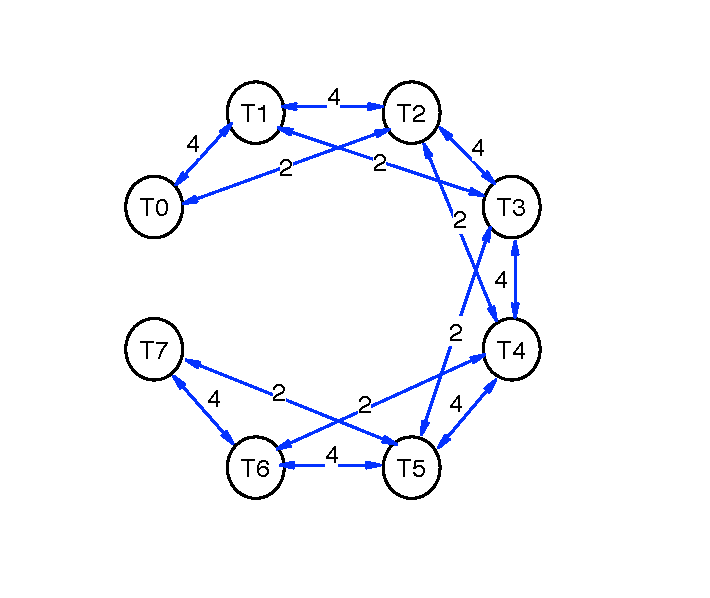
\includegraphics[scale=.45]{figs/Fig1a.pdf}
			%\caption{fig1}
		\end{minipage}%
	}%
	\subfigure[Communication matrix]{
		\begin{minipage}[t]{0.45\linewidth}
			\centering
			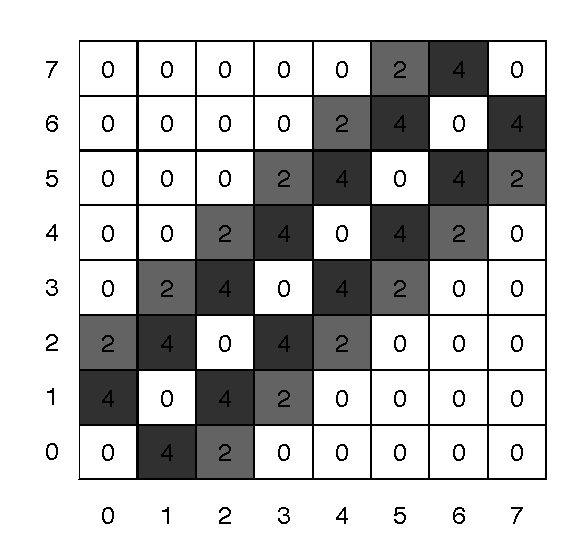
\includegraphics[scale=.45]{figs/Fig1b.pdf}
			%\caption{fig2}
		\end{minipage}%
	}%
	\centering
	\caption{An example of communication graph and communication matrix.} \label{FIG:1}
\end{figure}

Communication behavior of an application can be represent as a communication graph or task integration graph \cite{17}. Communication graph can be converted into a matrix, which contains the amount of communication between thread pairs where the indices represent the thread IDs, the communication matrix is symmetric and has a zero diagonal, as shown in Figure \ref{FIG:1}. CMLB and other communication-based mapping methods analyze the matrix to group threads and map them to machine.


We use CommDetective tool to detect the communication and generate the communication matrix. CommDetective is based on Linux Perf tools, and use the perf\_event\_open() system call to extract the memory access events from hardware performance monitoring unit (PMU). PMUs can be configured to trigger an overflow interrupt once a threshold number of events elapse. A PMU interrupt is referred to a “sample”, and Intel’s Precise Event-Based Sampling (PEBS) \cite{18} facility offers the ability to inspect the effective address accessed by the instruction on an event overflow for certain kinds of events such as loads and stores.  When two access events have the same access address, we consider the two events occur a communication, and update it in the communication matrix.

In this paper, we set perf\_event\_open() in CommDetective to perform sampling with sample frequency 1000 that means this tool will extract a sample from PMU every 1000 access events elapse, and set CommDetective to monitor two type of events for sampling: all loads micro operations and all stores micro operations.

\subsubsection{Analyzing the memory access load of each thread}
Diffierend from communication matrix, access load vector represents the memory access load of each thread. If a thread access the memory many times in the whole execution, it will has a high value in the access load vector. Therefore a high value in the access load vector imply the thread will make lots of pressure on memory. The whole process of analyzing the access load is divided into two parts: select and record all the DRAM access events in an access table, and analyze the access table using data analyzing methods to generate the access load vector.

We firstly select the events which access DRAM due to L3 cache miss when Perf extracts the samples of access events in CommDetective. That is because the access events which really access the DRAM could show the memory load feature acscurately, and the types of the events which selected are LLC\_MISS\_RETIRED.LOCAL\_DRAM, LLC\_MISS\_RETIRED.REMOTE\_DRAM. For each event we extract the related information include access address, thread id and the timestamp of accessing, and then make up these pieces of information to a record which will be stored at an access table. 

Secondly, we use the Pandas tool supported by Python to analyze the access table. The timestamp of each access record is converted to the time in nanoseconds (ns) according to the CPU clock frequency, the new timestamp is calculated by Equation \ref{equ1}

\begin{equation} \label{equ1}
	tsc=\frac{cycles\times1000000}{feq}
\end{equation}where $cycles$ represents the old timestamp in CPU clock cycles, and $feq$ represents the CPU clock frequency in khz. After the conversion is completed, a time slice needs to be set to merge the records whose timestamp interval is within it, and we set the time slice to 1ms in this paper. The merged record includes the timestamp, the thread id list, and the number of the original records which indicates how many memory accesses are performed in this time slice, and the higher this value, the higher the memory access data traffic in this time slice, and the higher the memory load. Therefore, it is necessary to focus on extracting the memory access feature of the merged records with a high number of original records, because these records will have a large impact on DRAM and are likely to cause memory congestion problem.

And then we can find the number of memory access changed regularly over time, as shown in Figure \ref{FIG:2}. We tested four applications, and plotted the timestamp, the amount of memory access of each merged record for every application in pictures. It’s easy to see that the time interval which has the large amount of memory access is likely to cause memory congestion, so we should focus on extracting each thread access load feature in that time interval. And there are some phases where the amount of access first increases and then decreases over the whole execution , so we need to divide the execution into several phases and combine the access load features from all the phases. 

\begin{figure}[htbp] 
	\centering	
	\subfigure[SP-OMP]{
		\begin{minipage}[t]{0.45\linewidth}
			\centering
			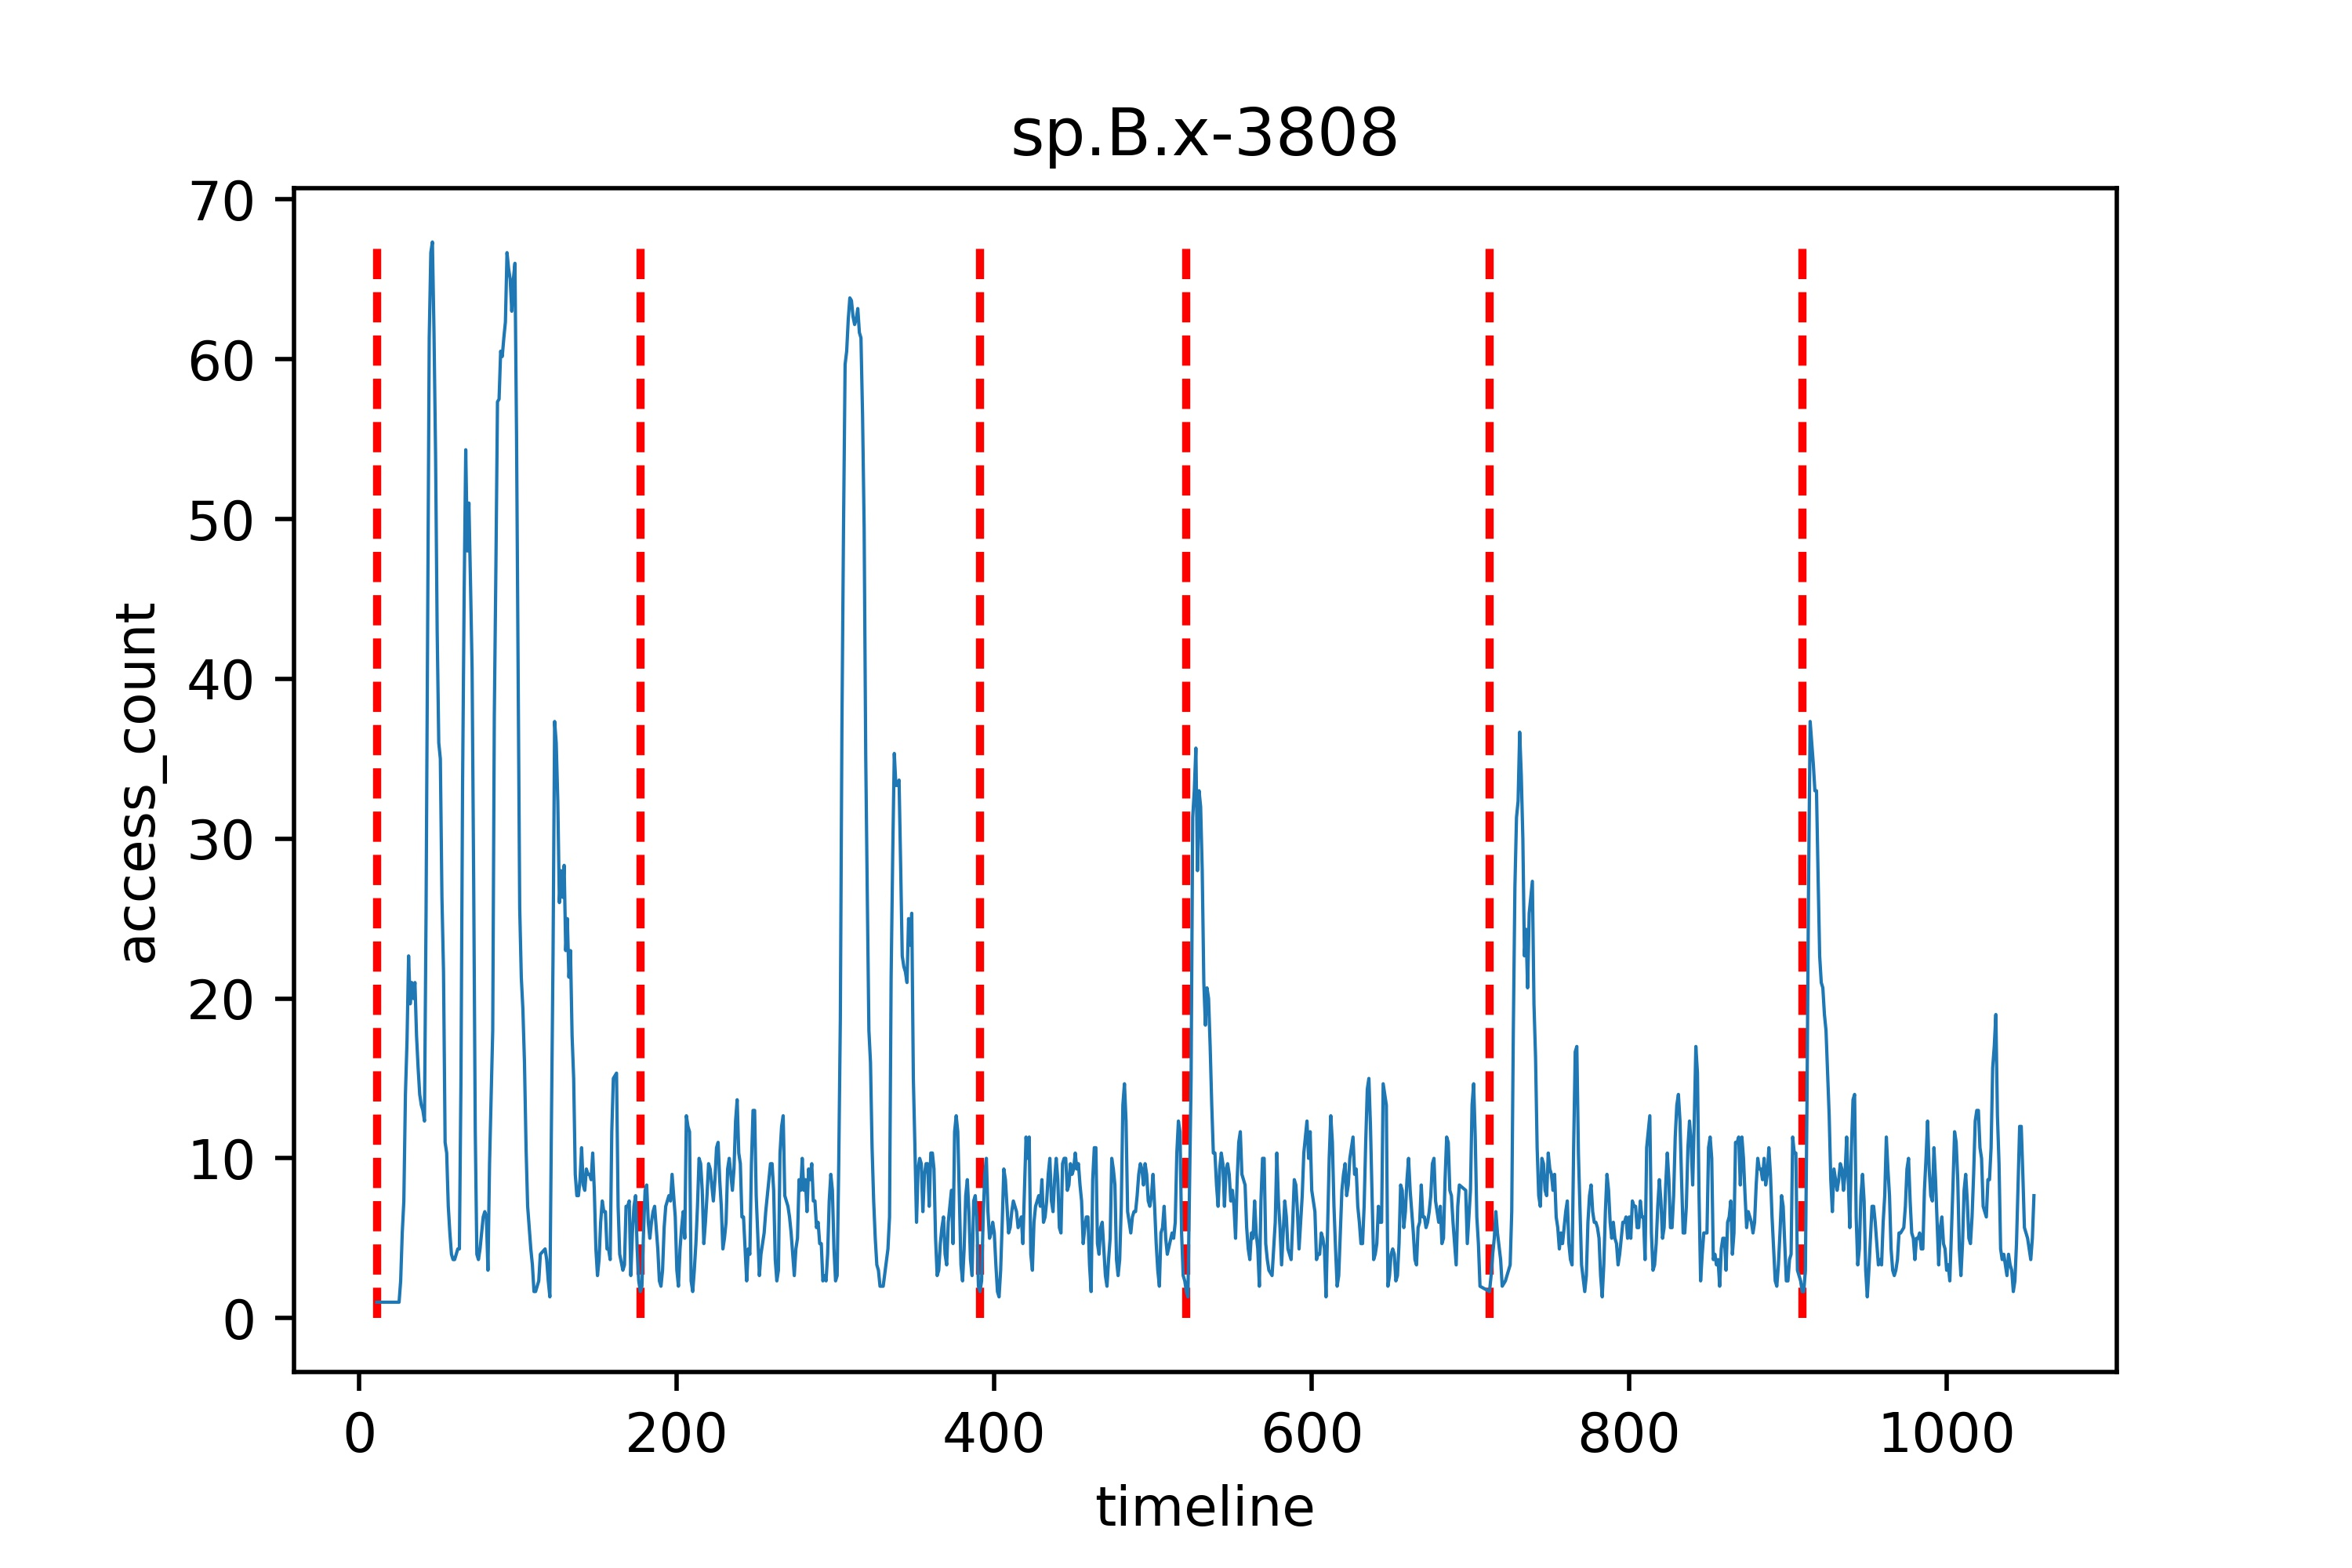
\includegraphics[scale=.40]{figs/Fig2a.jpg}
			%\caption{fig1}
		\end{minipage}%
	}%
	\subfigure[BT-OMP]{
		\begin{minipage}[t]{0.45\linewidth}
			\centering
			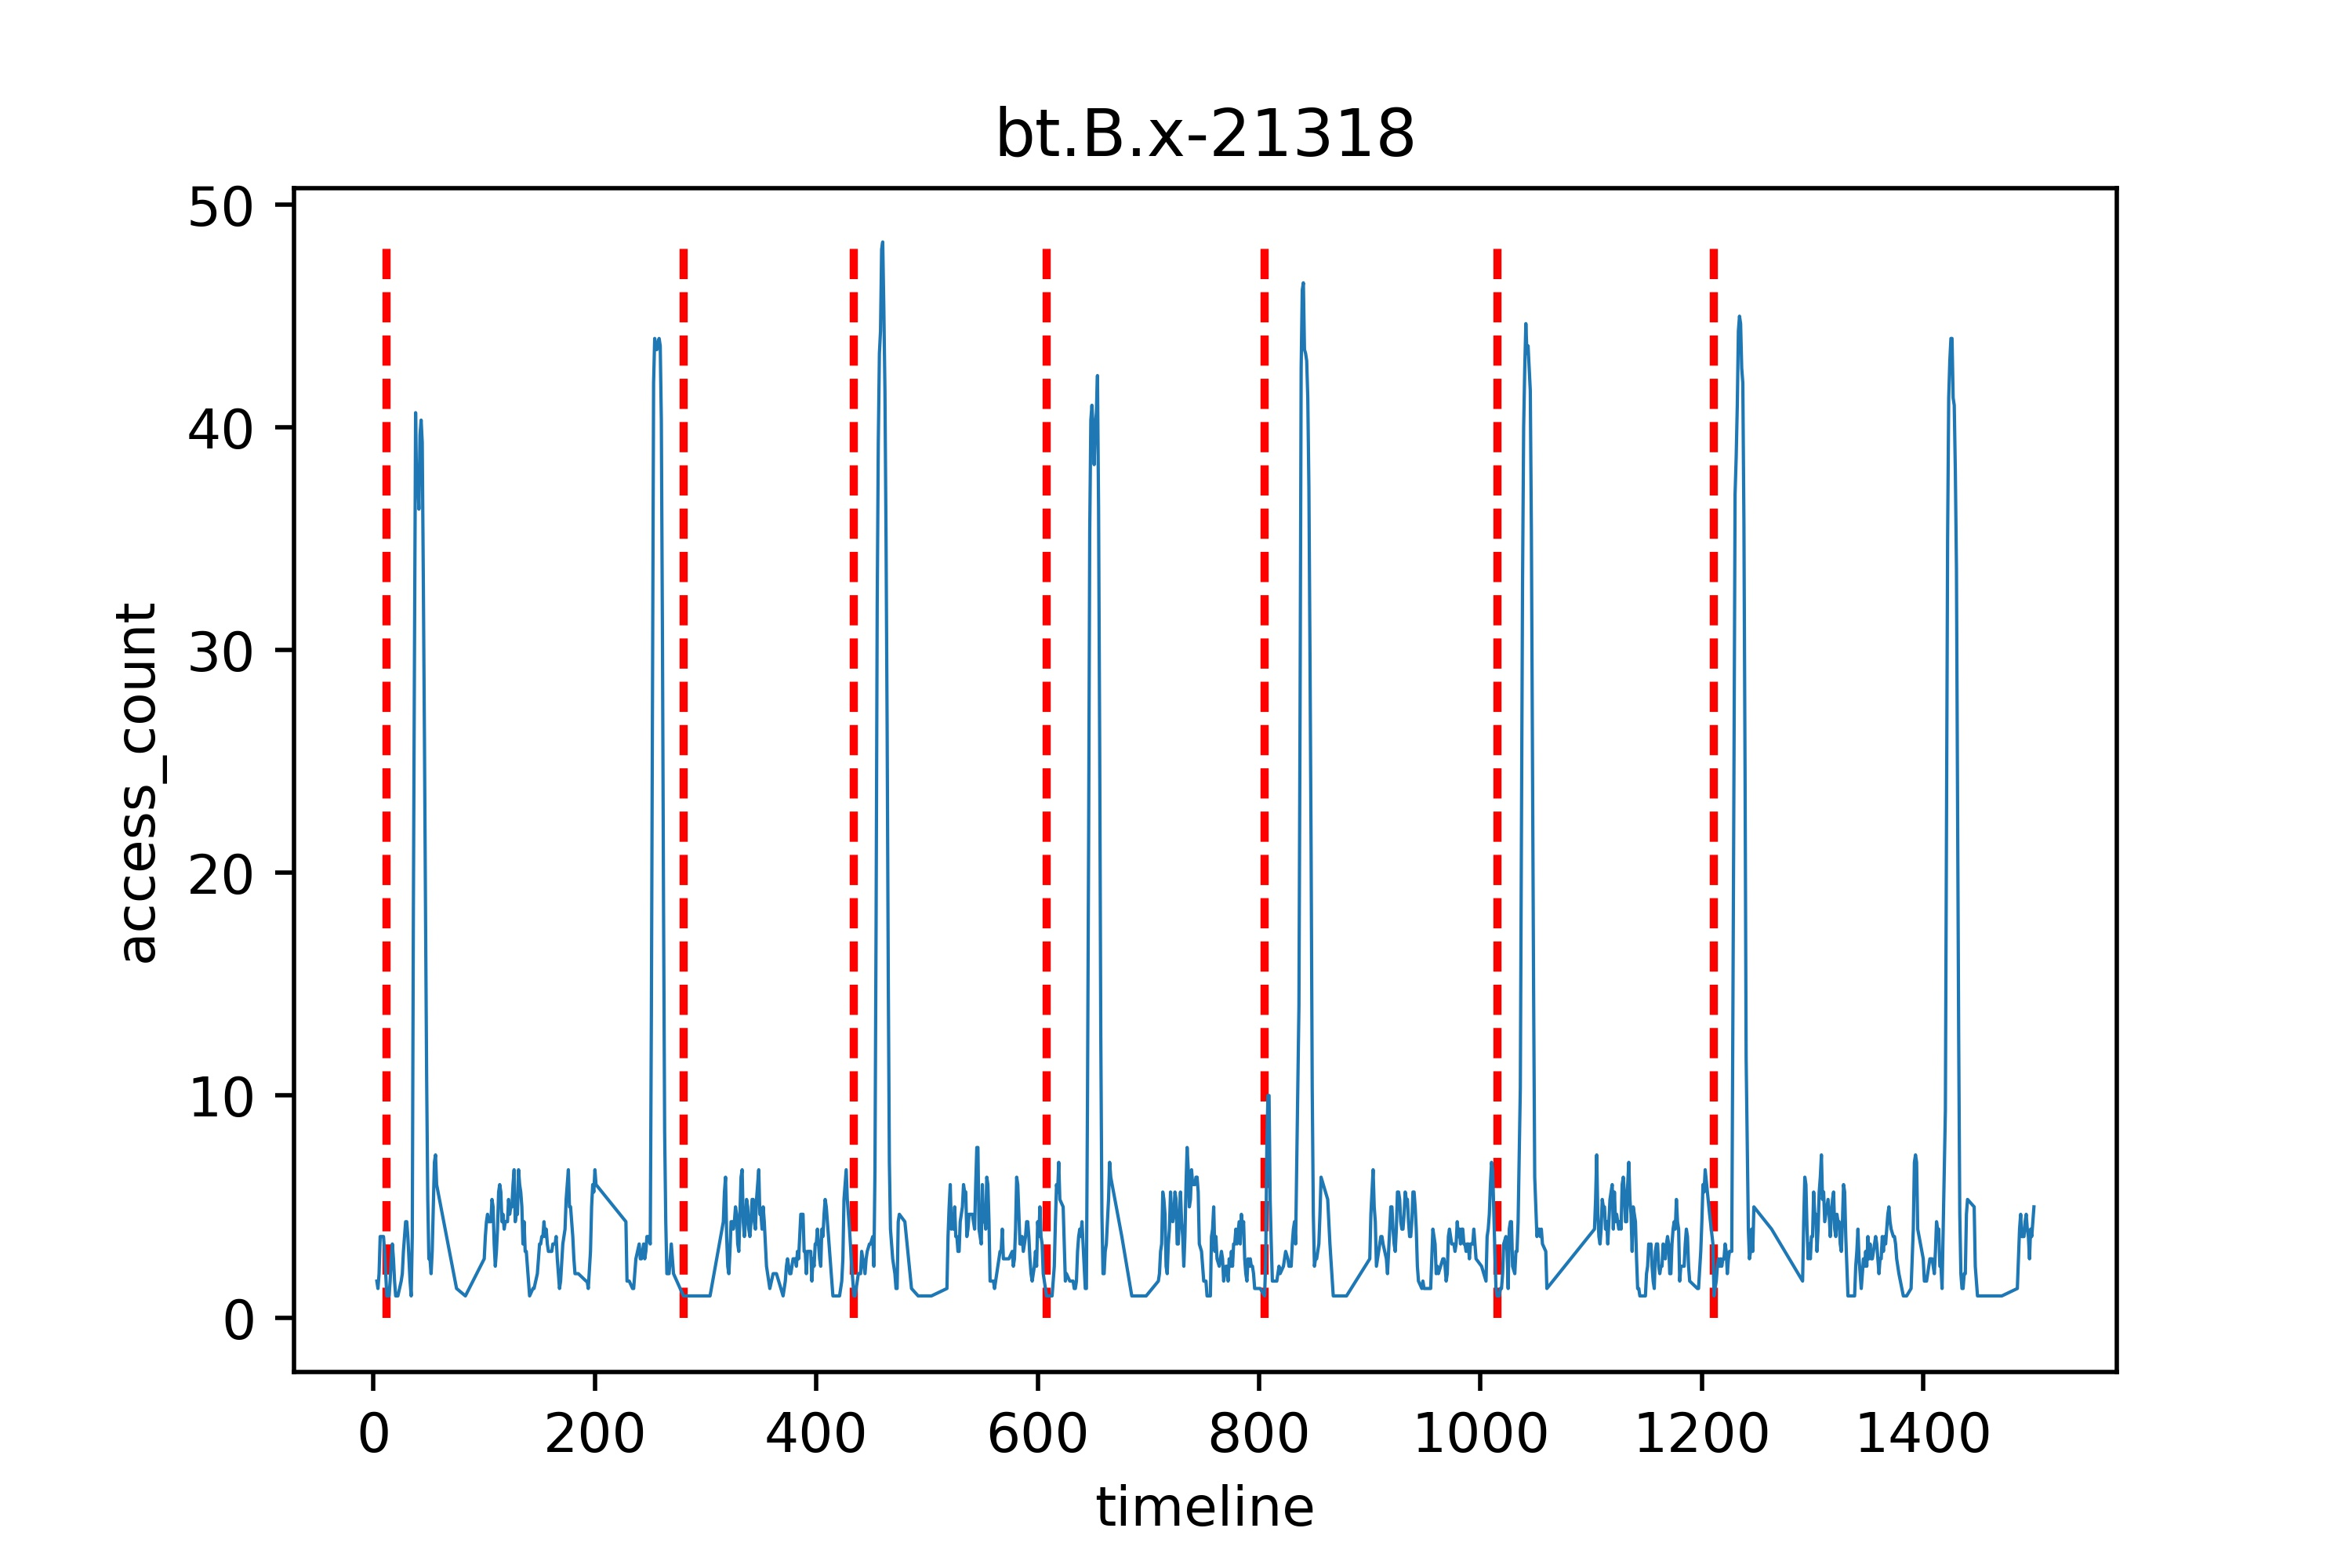
\includegraphics[scale=.40]{figs/Fig2b.jpg}
			%\caption{fig2}
		\end{minipage}%
	}%
	\, %这个回车键很重要 \quad也可以
	\subfigure[CG-OMP]{
		\begin{minipage}[t]{0.45\linewidth}
			\centering
			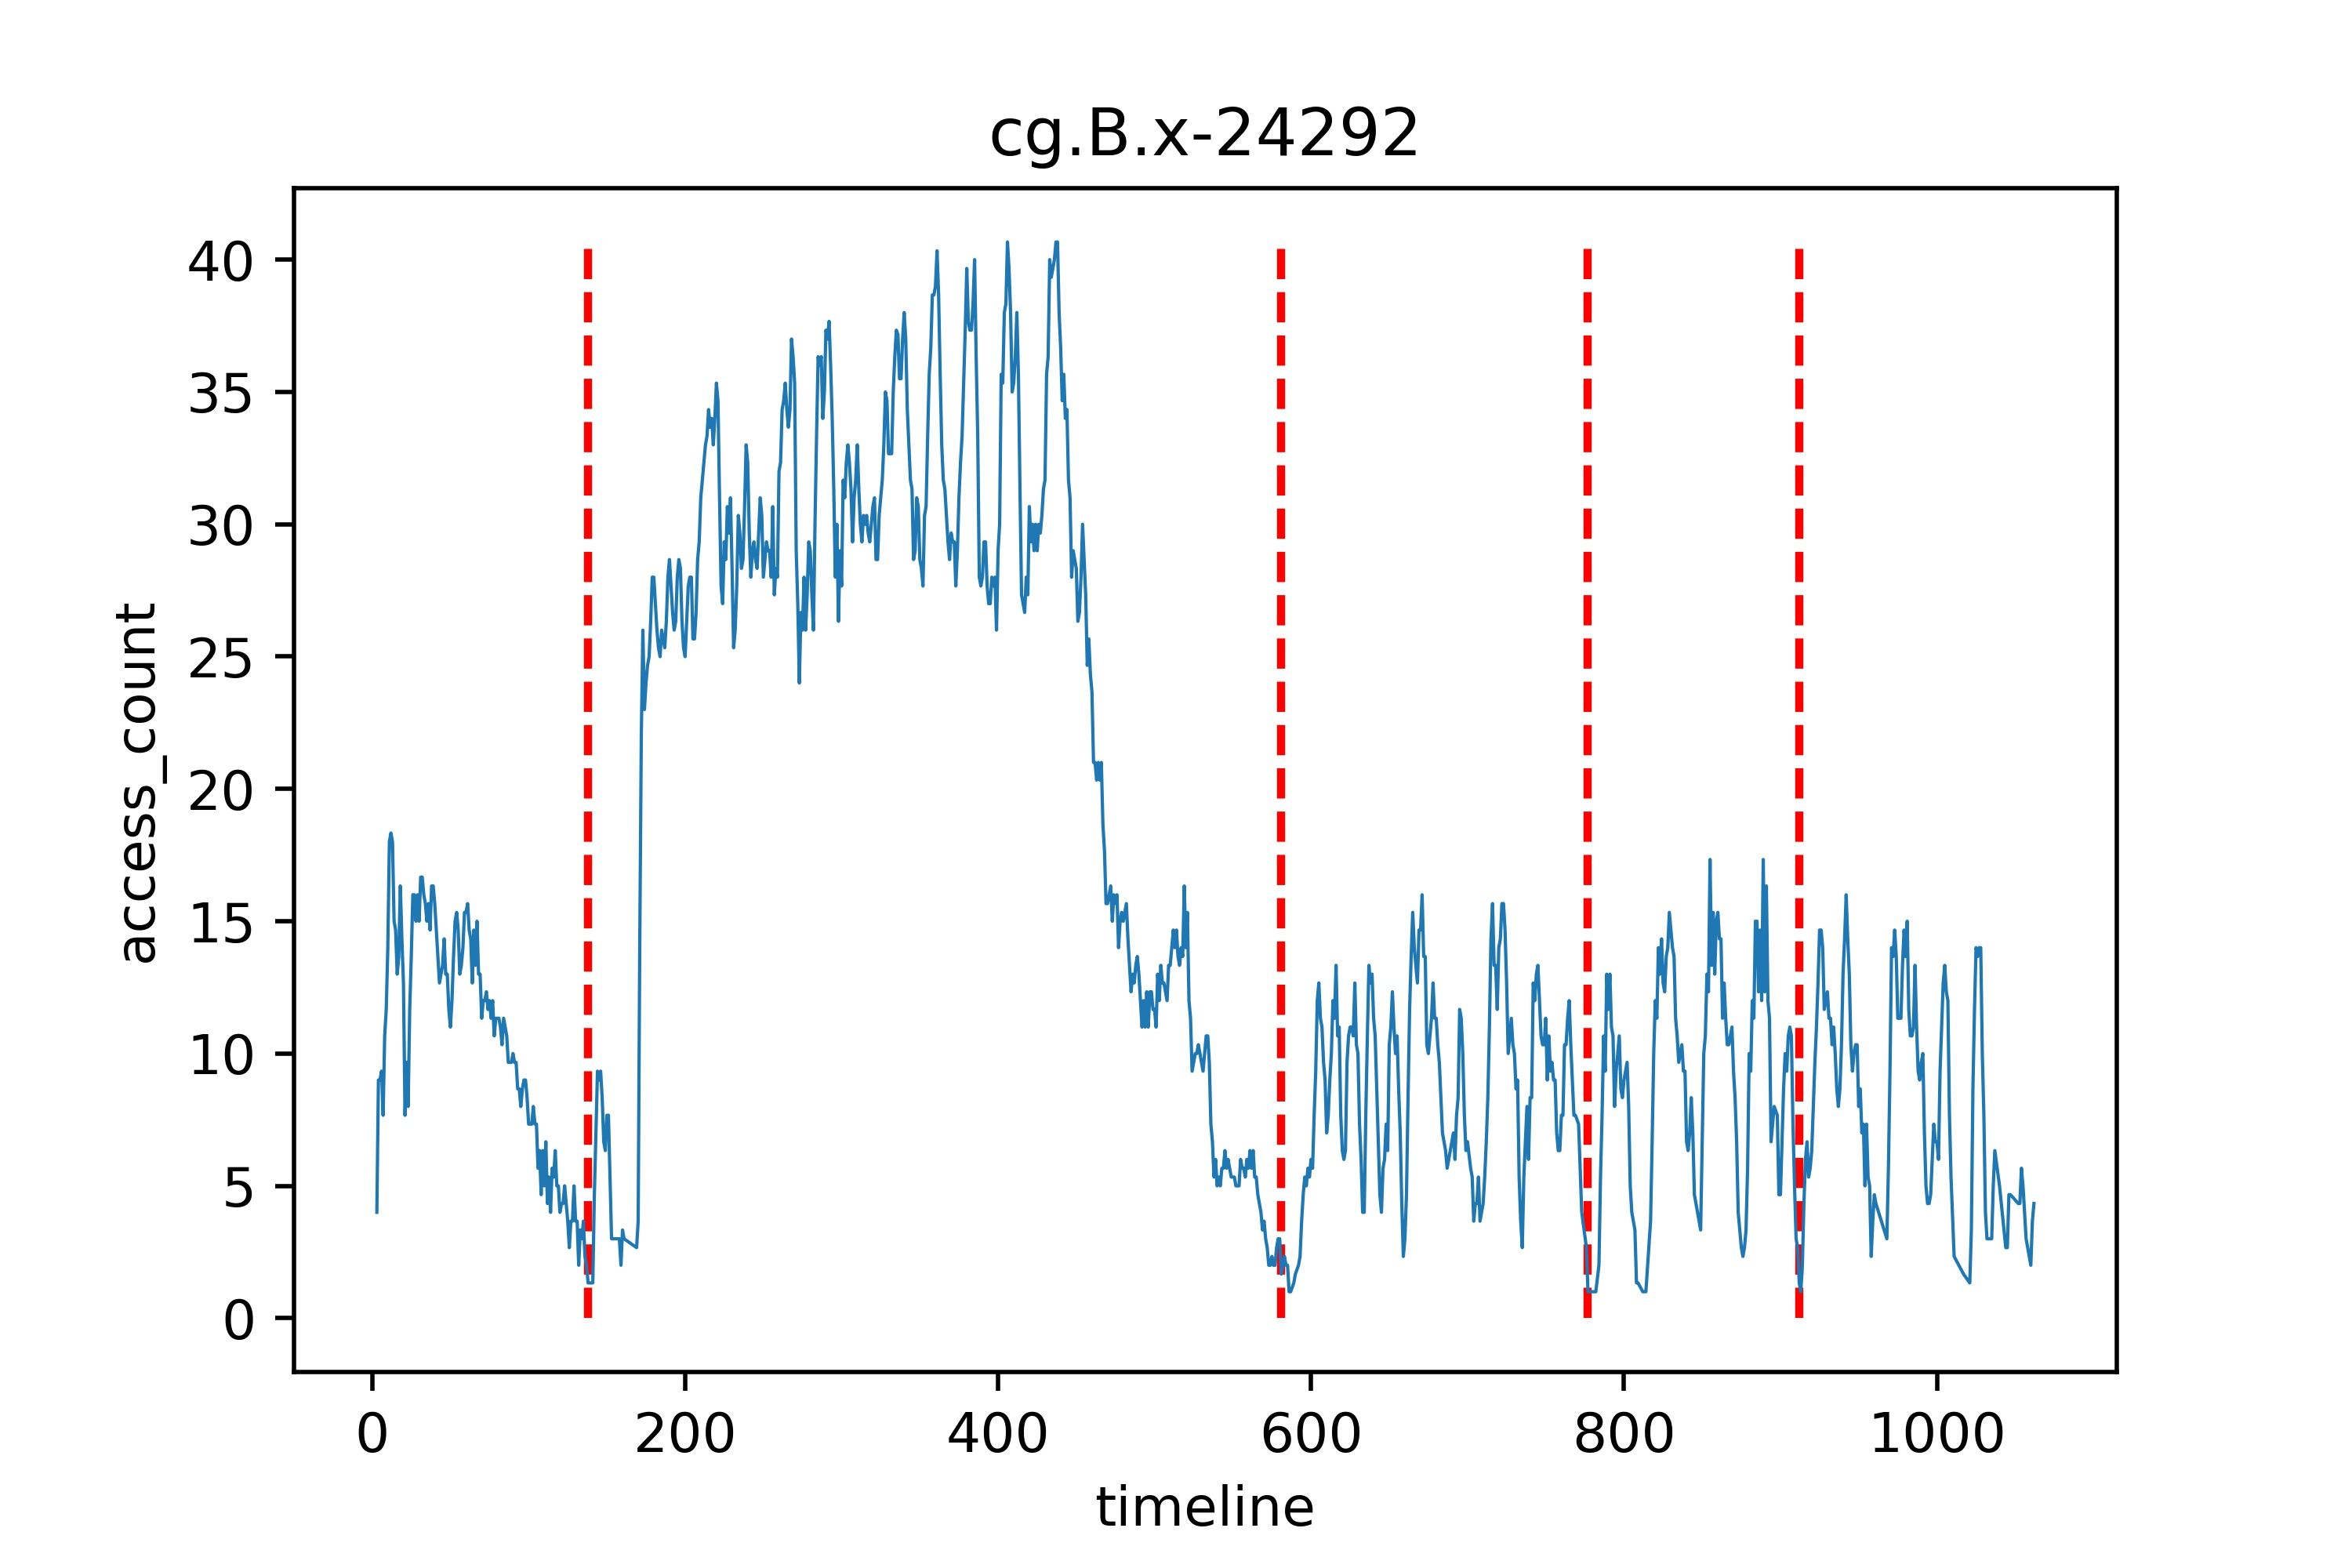
\includegraphics[scale=.40]{figs/Fig2c.jpg}
			%\caption{fig2}
		\end{minipage}
	}%
	\subfigure[LU-OMP]{
		\begin{minipage}[t]{0.45\linewidth}
			\centering
			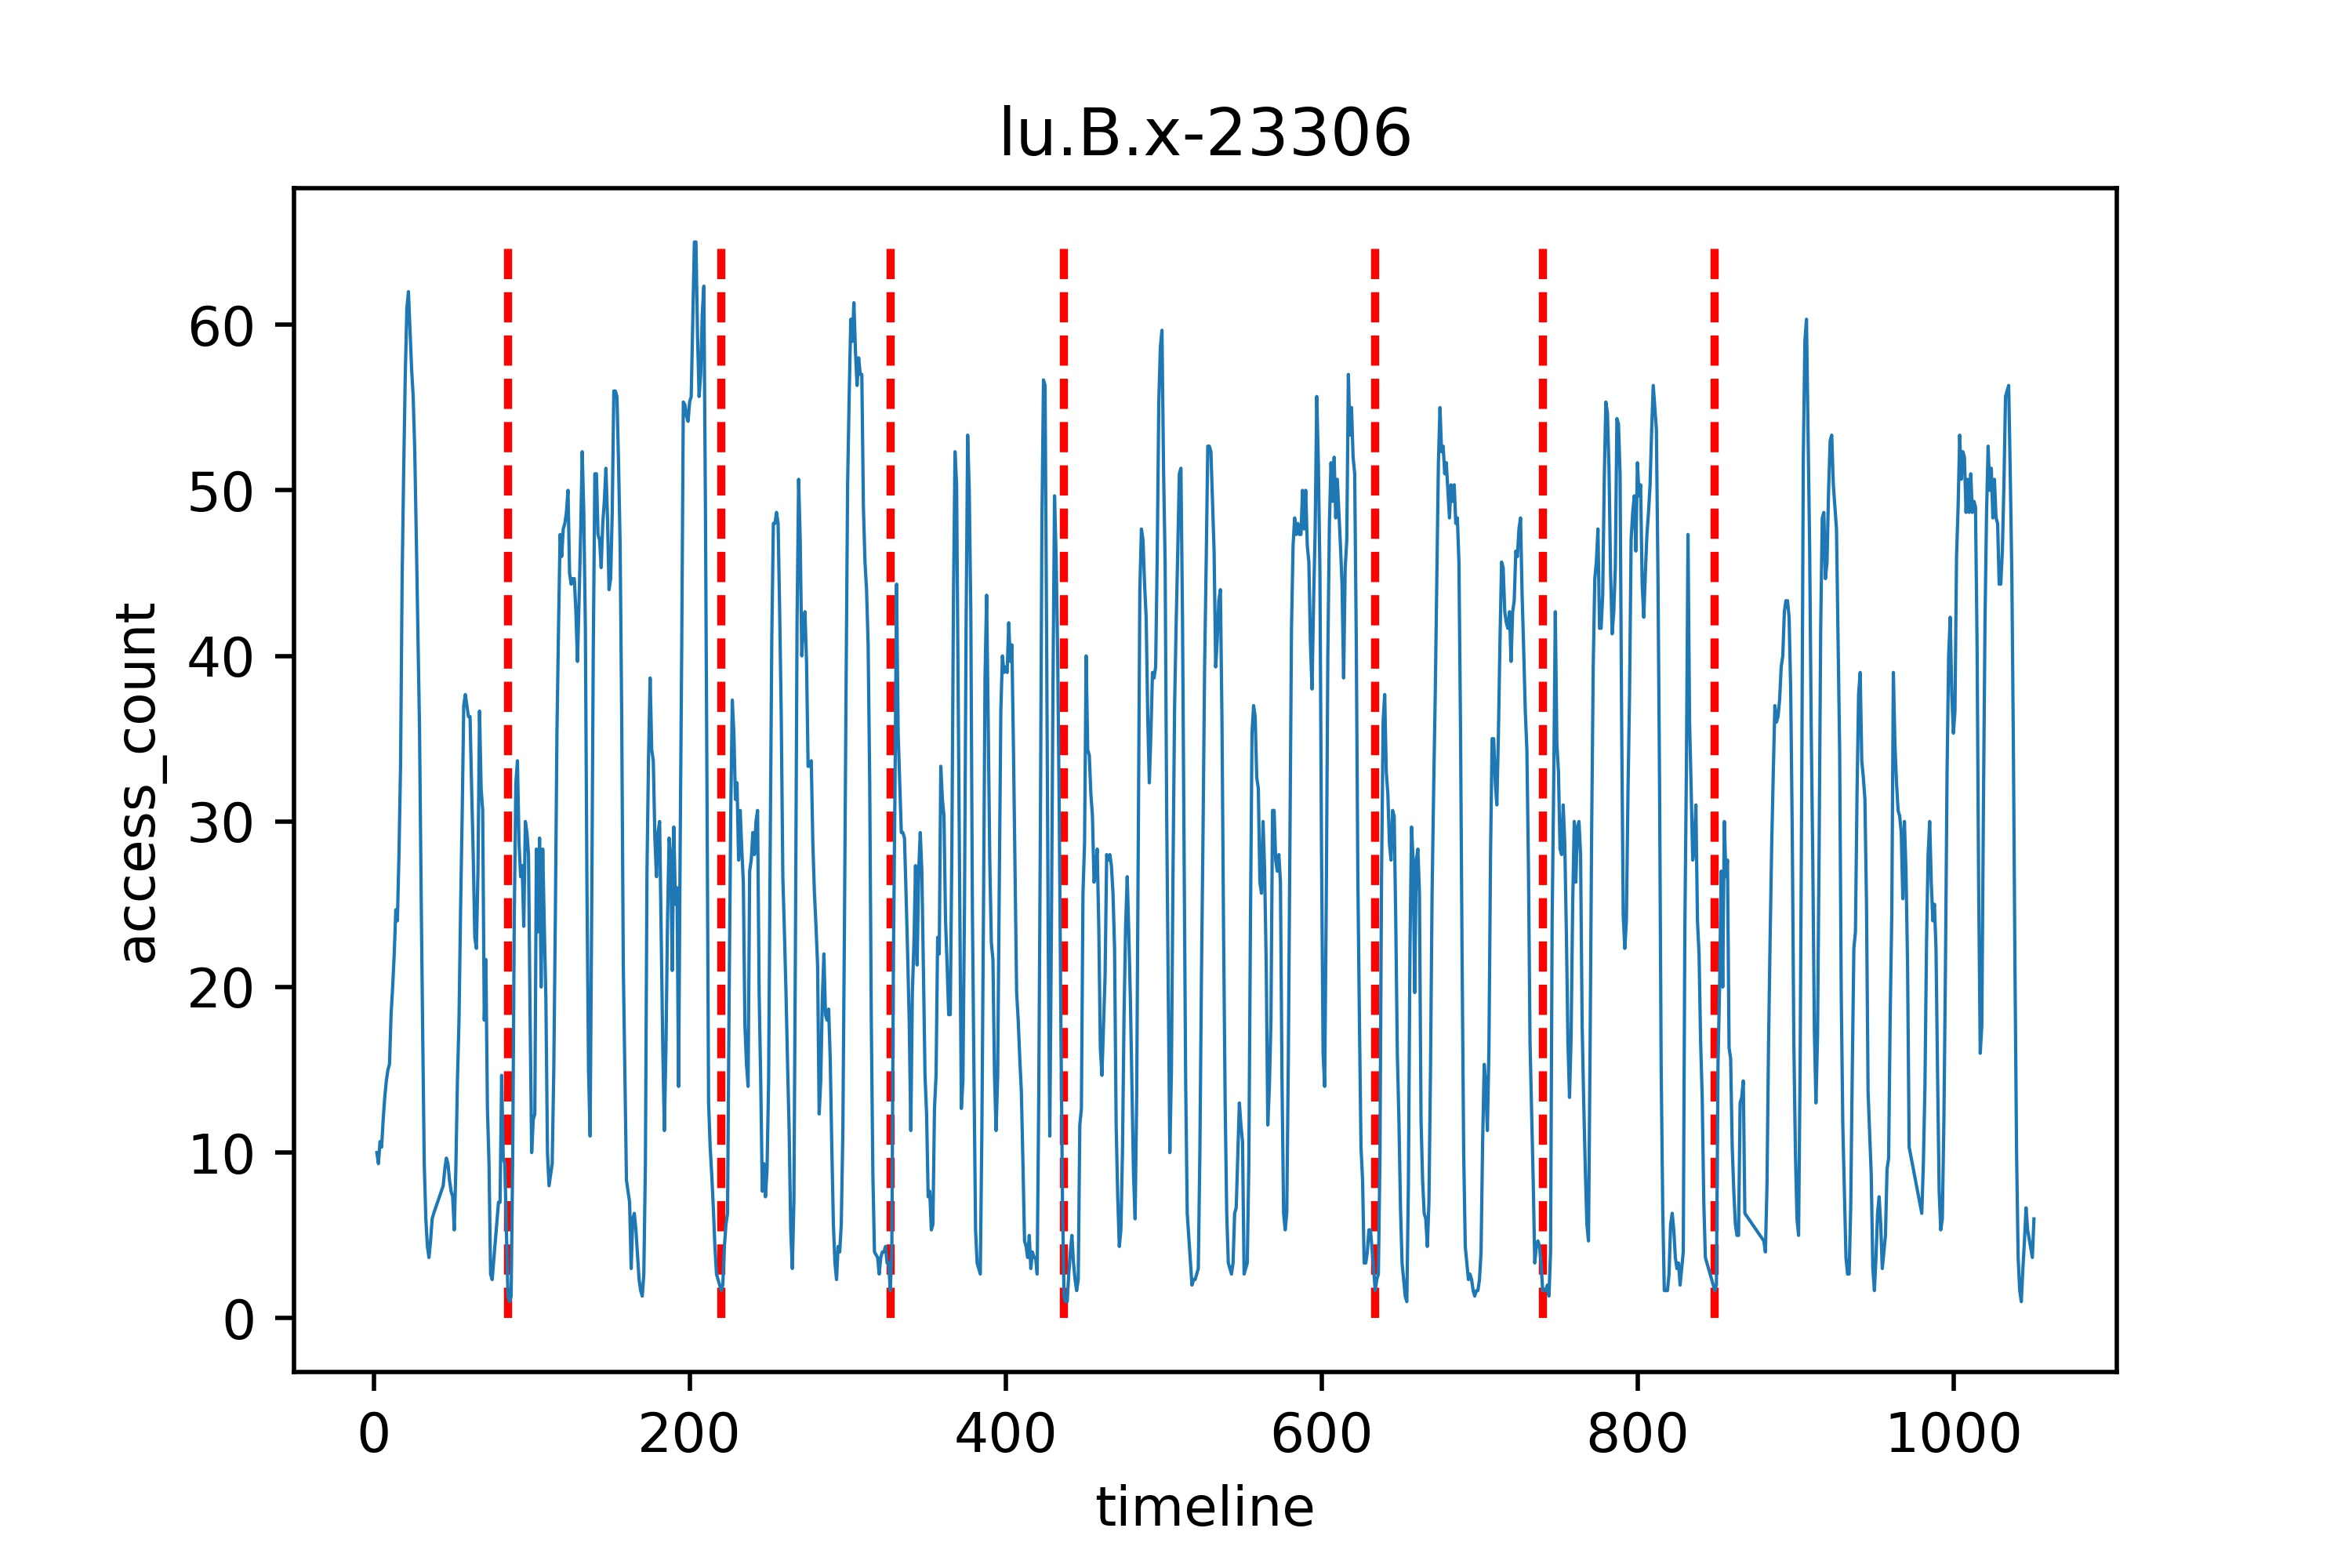
\includegraphics[scale=.40]{figs/Fig2d.jpg}
			%\caption{fig2}
		\end{minipage}
	}%
	
	\centering
	\caption{The time series of access amount in NPB benchmark} \label{FIG:2}
\end{figure}

We propose an access phases division algorithm based on the slide window algorithm, as shown in Algorithm \ref{alg1}, Before dividing the access phases, we firstly process the time series of the access amount. When using Perf to extract the access events, there may have noise to influence the data of time series. Therefore, we should linear smooth the time series of the access amount. According to the method in Rocka \cite{19}, the outliers in the time series data are usually less than 5\%, so we delete the data with the top 5\% of the value in the series, and use linear interpolation to fill in and replace. After smoothing the data, we use Algorithm \ref{alg1} to divide the access into phases. As Algorithm \ref{alg1} shown, we input the time series of the access amount which are linear smoothed, and use the means of the last 5\% of the value in the series as the low value of the access amount, which is shown from line 1 to line 2. And then, we set two pointers in line 3, and also set a  minimum window width in line 4 which represents the minimum time interval of an access phase. After that, we move forward the right pointer, when the right pointer meet the point with the low value, record the phase from left pointer to right pointer, and move the left pointer to the position of the right pointer for the next search.

\begin{algorithm}
\caption{Access phases disvsion}  \label{alg1}%算法的名字
\hspace*{0.02in} {\bf Input:} %算法的输入, \hspace*{0.02in}用来控制位置,同时利用 \\ 进行换行
s \{the time series of the access amount\}\\
\hspace*{0.02in} {\bf Output:} %算法的结果输出
phases \{the phases of the memory access\}
\begin{algorithmic}[1]
\State num = len(s) \times0.05$
\State low\_value = mean(sorted(s)[:num])
\State left = 0 ; right = 0
\State min\_width = 100
\While{right <= len(s)} {% While语句,需要和EndWhile对应
 	\If {s[right] <= low\_value and right - left >= min\_width} 
	 	\State phases.append(s[left : right+1])
 		\State left=right
	\EndIf 
	 \State right+=1
\EndWhile
\State \Return phases
\end{algorithmic}
\end{algorithm}

For practical considerations, there may have some small phases due to many continuous points with low value in the series, so minimum window width needs to be set to avoid existing too many small phases which will influence the result. In this paper, we set the minimum window width to 100, that means a phase has at least 100 time slices. By using Algorithm \ref{alg1}, we finally get all the access phases from an application. As shown in Figure \ref{FIG:2}, we tested four applications in NAS Parallel Benchmark (NPB), and the area between the red lines represents an access phase.

Due to each access phase has its own access load feature, we should extract the access load feature of each phase and combine them together. The access load feature of each phase could represent by a vector which include the access load of  each thread. In order to get the access load feature of a phase, we use the thread list in a merged record which represents the thread ids accessing the memory. And a phase includes at least 100 merged records, we merge all the thread list in a phase and count the access amount of each thread. 

Different phases have the different access amount, and the phase which has the large access amount will have a significant impact on memory access and be likely to cause memory congestion, so we use the average of access amount of a time slice in a phase to represent the weight of this phase. And then we use the weight of each phase to combine them, as shown in Equation \ref{equ2} and Equation \ref{equ3}.

\begin{equation} \label{equ2}
	w = \frac{1}{n} \sum_{i=1}^{n}d_i
\end{equation}
\begin{equation} \label{equ3}
	AccVector =\sum_{i=1}^{n}w_i . p_i
\end{equation}Equation \ref{equ2} calculate the weight of a phase, where $n$ represents the number of time slices in this phase and $d_i$ represents the access amount of the $i^{th}$ time slice, so $w$ represents the average of access amount of a time slice in this phase. And Equation \ref{equ3} calculate the final access load vector, where $n$ represents the number of the phases, $w_i$  represents the weight of the $i^{th}$ phase, and $p_i$ represents the access load vector of the $i^{th}$ phase.

\subsection{Computing and Grouping Threads}
\subsubsection{Description of Thread Grouping Algorithm}
According to section 1, CMLB is designed to work on improving the locality of communication as well as avoiding memory congestion problem. Therefore, the design principle of the grouping algorithm is to improve the locality of the memory access and ensure that the memory access load of each NUMA node is balanced. And we design the thread grouping algorithm using a top to bottom mode.

\begin{algorithm}
\caption{Top-Level Algorithm}  \label{alg2}%算法的名字
%算法的输入, \hspace*{0.02in}用来控制位置,同时利用 \\ 进行换行
\hspace*{0.02in} {\bf Input:} CommMat \{the communication matrix\} \\
\hspace*{0.02in} {\bf Input:} AccVector \{the access load vector\} \\
\hspace*{0.02in} {\bf Input:} configMap \{ the machine components topology\} \\ 
\hspace*{0.02in} {\bf Output:} %算法的结果输出
map\_res \{the result of threads grouping\}
\begin{algorithmic}[1]
\State num\_nodes = configMap[‘nodes’]
\State num\_threads = len(CommMat)
\State per\_group\_tids = num\_threads // num\_nodes
\State map\_res = []; overLoad\_list = []
\State last\_threads = [x for x in range(num\_threads)]
\For {i in range (num\_nodes)}
\State group, last\_threads = GenerateOneGroup(per\_group\_tids, last\_threads) 
\State map\_res.append(group)
\EndFor
\State \Return map\_res
\end{algorithmic}
\end{algorithm}

We firstly determine the number of groups of all threads, and generate all the groups in a loop. In order to make full use of the computing resources, all the running threads are distributed on all NUMA nodes. Therefore, the number of the groups of threads is the number of NUMA nodes. With hwloc \cite{20} tool, we can get the machine components topology including the number of nodes, the number of cores and memory caches in each node. As Algorithm \ref{alg2} shown, we input the communication matrix, access load vector and the configure map which records the machine topology, and then calculate the number of threads in each group and initialize variables such as the list of threads to be grouped and the list of grouping results from line 1 to line 5. From line 6 to line 8, generate each group and add the result of each group to the final result list. At last, return the result of threads grouping in line 10. 


The function GenerateOneGroup which represents the process to generate a group of threads is described in Algorithm \ref{alg3}. According to Algorithm \ref{alg2}, we get the number of  threads for a group, and then select a thread from the list of the remaining threads. And repeat the above step until the number of threads in the group reaches the upper limit. As Algorithm \ref{alg3} shown, we firstly input the number of threads in each group and the list of the remaining threads to be grouped, then initialize the group list and update the remaining list to be grouped from line 1 to line 2. And select one of the remaining threads to be grouped to insert and update the remaining list from line 3 to line 6. At last, return a group of threads and the remaining threads list in line 8. 

\begin{algorithm}
\caption{GenerateOneGroup} \label{alg3}%算法的名字
%算法的输入, \hspace*{0.02in}用来控制位置,同时利用 \\ 进行换行
\hspace*{0.02in} {\bf Input:} per\_group\_tids \{the number of threads in each group\} \\
\hspace*{0.02in} {\bf Input:} last\_threads \{list of remaining threads to be grouped\} \\
\hspace*{0.02in} {\bf Output:} %算法的结果输出
group \{a group of threads\} \\
\hspace*{0.02in} {\bf Output:} last\_threads \{list of remaining threads to be grouped\} 
\begin{algorithmic}[1]
\State group = last\_threads[0]
\State last\_threads.pop(); overLoad\_list.clear()
\For {i in range (per\_group\_tids)}
\State tar\_tid = SelectOneThread(cur\_grouped ,last\_threads)
\State group.append(tar\_tid)
\State last\_threads.remove(tar\_tid)
\EndFor
\State \Return group, last\_threads
\end{algorithmic}
\end{algorithm}
In order to implement the function SelectOneThread in line 4 of Algorithm \ref{alg3}, we reference the greedy policy in EagerMap. According to the list of grouped threads $t$ = [t_1,t_2,t_3]$ and the communication matrix, we calculate all the amount of communication between all the remaining threads and $t$, and sort the communication from high to low. We select each thread t_w$ from all the remaining threads and calculate the sum of communication with all the threads in $t$, as shown in Equation \ref{equ4}

\begin{equation} \label{equ4}
	C = \sum_{i=1}^{n}$CommMatrix$[t_w][t[i]]
\end{equation}Where $Commmatrix$ represents the communication matrix, $n$ represents the number of grouped threads in $t$, and $C$ represents the sum of the communication between one remaining thread t_w$ and all the threads in $t$. And then we can calculate all the sum of communication between the remaining threads and $t$, and sort them from high to low. At last, we get the communication rank list:[[$C_1$, t_w_1], [$C_2$,t_w_2], …]$. When selecting a thread to insert in the group, we can visit the communication rank list and choose the first element where the thread has the largest communication amount with all the grouped threads, and then check that if inserting the t_w_1$ will destroy the memory access balance in this group according to access load vector. If it not, inserting t_w_1$ in the group will be safe, otherwise, choose the next thread t_w_2$ in the communication rank list and repeat the above steps until select a thread to insert in the group. The method of judge the balance of the access load in a group will described in next part.

\begin{algorithm}
\caption{SelectOneThread} \label{alg4}%算法的名字
%算法的输入, \hspace*{0.02in}用来控制位置,同时利用 \\ 进行换行
\hspace*{0.02in} {\bf Input:} cur\_grouped \{the list of grouped threads\} \\
\hspace*{0.02in} {\bf Input:} last\_threads \{the list of remaining threads\} \\
\hspace*{0.02in} {\bf Output:} %算法的结果输出
tar\_tid\{the thread selected to be grouped\}
\begin{algorithmic}[1]
\State rank\_ls = []
\For {last\_t in last\_threads}
\State sum\_ = 0
\For {grouped\_t in cur\_grouped}
\State sum\_ += CommMat[grouped\_t][last\_t]
\EndFor
\State rank\_ls.append([sum\_, last\_t])
\EndFor
\State rank\_ls = sorted(rank\_ls, reverse=True)
\For {pair in rank\_ls}
\If {JudgeLoadBalance(pair[1], cur\_grouped, last\_threads)}
\State \Return pair[1]
\EndIf 
\EndFor
\State \Return rank\_ls[0][1]
\end{algorithmic}
\end{algorithm}

As the Algorithm \ref{alg4} shown, we input the list of grouped threads and the list of remaining threads, and calculate the sum of the communication between each remaining thread and all the grouped threads and record in the rank list from line 1 to line 8. And then visit the rank list and choose the thread from line 9 to line 14. At last, return the grouped thread. Particularly, if all the threads in rank list destroy the balance of the group, the thread which is the first element in rank list will be selected.

\begin{algorithm}
\caption{JudgeLoadBalance}  \label{alg5} %算法的名字
%算法的输入, \hspace*{0.02in}用来控制位置,同时利用 \\ 进行换行
\hspace*{0.02in} {\bf Input:} tid\{the candidate thread \} \\
\hspace*{0.02in} {\bf Input:} cur\_grouped \{the list of grouped threads\} \\
\hspace*{0.02in} {\bf Input:} last\_threads \{the list of remaining threads\} \\
\hspace*{0.02in} {\bf Output:} %算法的结果输出
bool type
\begin{algorithmic}[1]
\State cur\_load = AccVector[tid]
\For {grouped\_t in cur\_grouped }
\State cur\_load += AccVector[grouped\_t]
\EndFor
\State last\_load = sum(AccVector) / num\_nodes - cur\_load
\State last\_num\_tids = per\_group\_tids – len(cur\_grouped)
\If {last\_num\_tids == 1 and tid in overLoad\_list}
\State\Return False
\Else
\State\Return True
\EndIf
\State f = sorted(last\_threads.remove(tid),reverse=True)
\State max\_load = sum(f[ : last\_num\_tids])
\State min\_load = sum(f[-last\_num\_tids:])
\If {last\_load >= min\_load and last\_load <= max\_load}
\State\Return True
\Else
\State\Return False
\EndIf
\end{algorithmic}
\end{algorithm}

According to the Algorithm  \ref{alg4}, before we select  thread to insert the group, we should check whether it will destroy the load balance of the group, and the function in line 11 of Algorithm  \ref{alg4} implement that. After determining the number of the groups in Top-Level Algorithm, we need to calculate the average memory load of each group according to the access load vector, as shown in Equation \ref{equ5}.

\begin{equation} \label{equ5}
	Aml =  \frac{1}{groups}\sum_{i=1}^{n}AccVector[i]
\end{equation}Where $groups$ represents the number of the groups, $n$ represents the length of the access load vector, and $Aml$ represents the average memory load of each group. 

When selecting a thread from the rank list, the thread $t_w$ insert the group at first, calculate the current load of this group and the $lastLoad$ which is the difference between $Aml$ and current load, and calculate $n$ which represents the number of the remaining threads in this group at the same time. After that, we sort all the remaining threads according to the value in the $AccVector$ from high to low, and calculate the $maxLoad$ and $minLoad$ which represent the sum of the access load of  the top $n$ threads and last $n$ threads after sorted. If $lastLoad$ is between $minLoad$ and $maxLoad$, the thread $t_w$ will not destroy the balance in this group. Otherwise, $t_w$ will destroy the balance. That’s because we can not find $n$ remaining threads to make the load reach $lastLoad$ and the total load of this group will also  not reach $Aml$. 

As Algorithm  \ref{alg5} shown, we input the candidate thread, the list of grouped threads and the list of remaining threads. From line 4 to line 6, calculate the current access load of this group, and then calculate $lastLoad$ and $n$ from line 5 to line 6. From line 12 to line 18, calculate $maxLoad$, $minLoad$ and check if $lastLoad$ is between $maxLoad$ and $minLoad$.

\subsubsection{An example of Grouping Threads}

\begin{figure}[htbp] 
	\centering	
	\subfigure[Input communication matrix and access load vector]{
		\begin{minipage}[t]{0.45\linewidth}
			\centering
			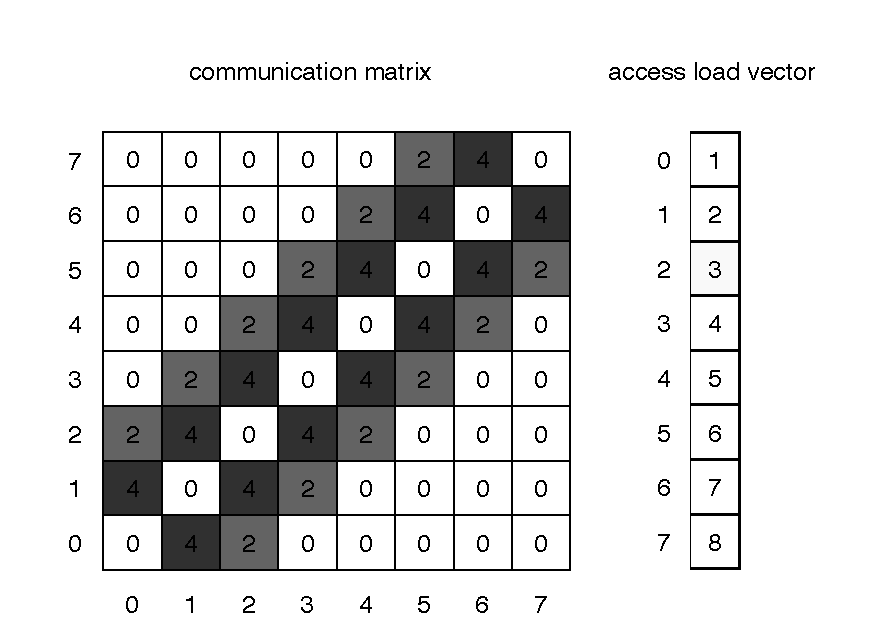
\includegraphics[scale=.40]{figs/Fig3a.pdf}
			%\caption{fig1}
		\end{minipage}%
	}%
	\subfigure[Judge access load balance when inserting a thread]{
		\begin{minipage}[t]{0.45\linewidth}
			\centering
			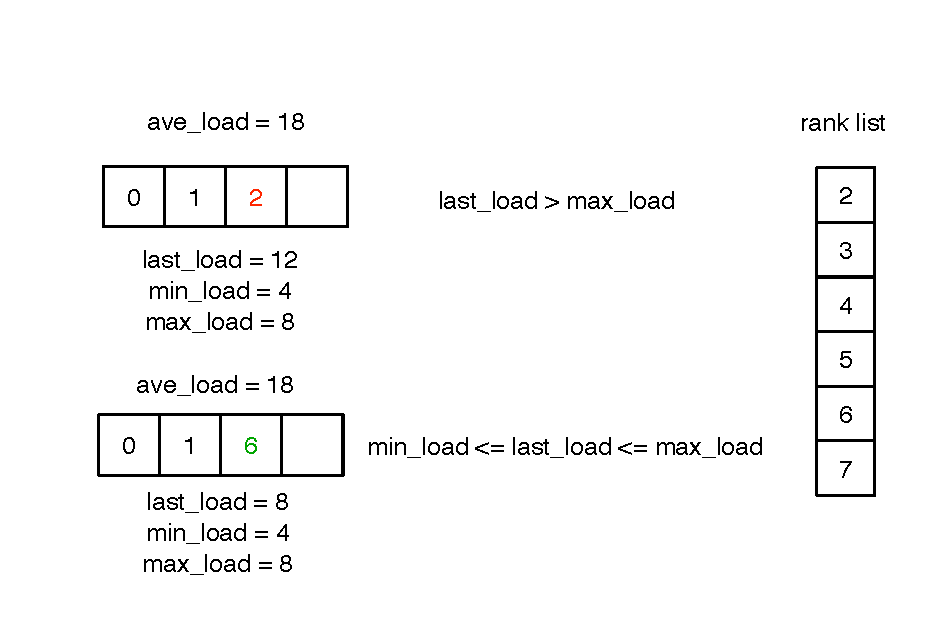
\includegraphics[scale=.40]{figs/Fig3b.pdf}
			%\caption{fig2}
		\end{minipage}%
	}%
	\, %这个回车键很重要 \quad也可以
	\subfigure[The result of grouping]{
		\begin{minipage}[t]{0.45\linewidth}
			\centering
			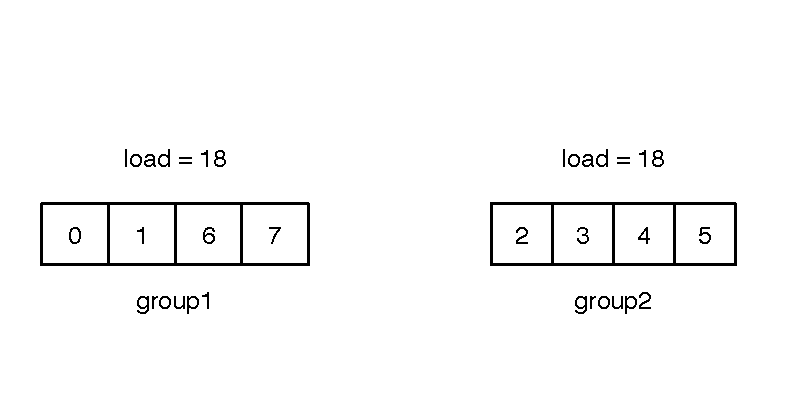
\includegraphics[scale=.43]{figs/Fig3c.pdf}
			%\caption{fig2}
		\end{minipage}
	}%
	\centering
	\caption{An example of grouping threads} \label{FIG:3}
\end{figure}

We now explain the thread grouping algorithm with an example shown in Figure \ref{FIG:3}. At the beginning, we input a communication matrix and an access load vector, and there are 8 threads in total. All the threads will be grouped into 2 groups due to our machine has 2 NUMA nodes, so each group has 4 threads. As shown in Figure 3b, the group 1 now has 2 threads (0 and 1), when selecting another thread to insert the group, we should judge the access load of the group.

Firstly, we sort all the remaining threads from high to low according to the communication with thread 0 and thread 1, and record them in the rank list. And then, choose the first element (thread 2) from the rank list and try to insert in the group. According to the access load vector, we can calculate $Aml$ is 18 ((1+2+ .. +8)/2) and $lastLoad$ is 12 due to the current load including thread 0,1,2 is 6. And we calculate minLoad which the remaining threads can provide is 4 (provided by thread 3), and we can also calculate $maxLoad$ is 8 (provided by thread 7). After that, we find lastLoad is larger than $maxLoad$, if thread 2 insert the group, the total load of this group will larger than $Aml$ and will make imbalance on two groups. Therefore, we choose next thread in rank list until find a proper thread. And finally we select the thread 6 that will not destroy the balance of groups. At last, thread 0,1,6 and 7 are grouped in group 1, and thread 2,3,4 and 5 are grouped in group 2, and we can find the total access loads of 2 groups are the same. 

\subsection{Theoretical  Evaluation of the Algorithm}
In this section, we will test the theoretical performance of CMLB and compare with the state-of-art mapping methods including EagerMap, TreeMatch and ChoiceMap from the amount of remote communication and the access balance of NUMA nodes.

After getting the mapping result from a mapping method, we can measure remote communication and the load balance of nodes according to the communication matrix and access load vector. Due to both of the mapping methods which we compare with are the communication-based methods, we can calculate the remote communication using the  communication matrix, as shown in Equation \ref{equ6} and Equation \ref{equ7}. 

\begin{equation} \label{equ6}
	RemoteComm =   \sum_{i=1}^{n}\sum_{j=i+1}^{n}CommVal(map[i],map[j])
\end{equation}

\begin{equation} \label{equ7}
	CommVal(g1,g2) =   \sum_{m=1}^{n1}\sum_{n=1}^{n2}CommMat[g1[m]][g2[n]]
\end{equation}In Equation 6, where $n$ represents the number of nodes and we regard the threads in a node as a group. $CommVal$ represents the function to calculate the communication between two groups and $map$ represents the mapping result of all the groups. Equation 7 is the process of calculating $CommVal$, where $g1$, $g2$ represent the two groups and $n1$, $n2$ represent the number of threads in the two groups. $RemoteComm$ corresponds to the QPI in section 4, the lower this value, the higher the performance gains.

The access load balance of the nodes is also a criterion to judge the performance of mapping method. It is measured by Equation \ref{equ8} and Equation \ref{equ9}.

\begin{equation} \label{equ8}
	Load_s_t_d =   \sqrt{\frac{\sum_{i=1}^{n}(L_i-L) }{n}}
\end{equation}

\begin{equation} \label{equ9}
	L_i = \frac{1}{m}\sum_{j=1}^{m}AccVector[L_i[j]]
\end{equation}In Equation 8, where $Load_s_t_d$ represents the standard deviation of the access load between groups, $n$ represents the number of the groups. And $L_i$ is the access load in the i^{th} group, L$ represents the means of the access load of all the groups. In Equation 9 is the process of calculate the $L_i$, $m$ represents the number of the threads in one group and Accvector is the access load vector. $Load_s_t_d$ corresponds to the imbalance in section 4, the lower this value, the higher the performance gains.

And then we test SP, BT and LU applications using the two metrics to compare the theoretical performance of CMLB with the other mapping methods. As shown in table1,2 and 3.

\begin{table}[width=.71\linewidth,cols=6,pos=h]
	\caption{The test result of SP-OMP}\label{tbl1}
	\begin{tabular*}{\tblwidth}{@{} LLL@{} }
		\toprule
		Method & RemoteComm & Load_s_t_d \\
		\midrule
		CMLB & 1.99 \times 10^8 &139.37 \\
		EagerMap & 1.90 \times 10^8 & 33455.01 \\
		TreeMatch & 2.13 \times 10^8 & 29343.56 \\
		ChoiceMap & 1.92 \times 10^8 & 33214.47 \\
		\bottomrule
	\end{tabular*}
\end{table}

\begin{table}[width=.71\linewidth,cols=6,pos=h]
	\caption{The test result of LU-OMP}\label{tbl1}
	\begin{tabular*}{\tblwidth}{@{} LLL@{} }
		\toprule
		Method & RemoteComm & Load_s_t_d \\
		\midrule
		CMLB & 3.51 \times 10^7 &462.69 \\
		EagerMap & 3.40 \times 10^7 & 29310.60 \\
		TreeMatch & 3.62 \times 10^7 & 28913.45 \\
		ChoiceMap & 3.54 \times 10^7 & 28712.68 \\
		\bottomrule
	\end{tabular*}
\end{table}

\begin{table}[width=.71\linewidth,cols=6,pos=h]
	\caption{The test result of BT-OMP}\label{tbl1}
	\begin{tabular*}{\tblwidth}{@{} LLL@{} }
		\toprule
		Method & RemoteComm & Load_s_t_d \\
		\midrule
		CMLB & 2.27 \times 10^8 &968.89 \\
		EagerMap & 1.89 \times 10^8 & 36440.19 \\
		TreeMatch & 2.01 \times 10^8 & 36642.56 \\
		ChoiceMap & 1.97 \times 10^8 & 35951.62 \\
		\bottomrule
	\end{tabular*}
\end{table}


From the tables we can see that, although CMLB is slightly higher than EagerMap, TreeMatch and ChoiceMap in $RemoteComm$ of  3 applications, they are all at an order of magnitude. As for $Load_s_t_d$ of 3 applications, CMLB is significantly lower than the other methods. CMLB could greatly reduce the difference of memory access load between nodes as well as the remote communication is not much higher than the other methods. Therefore, CMLB is better than the other mapping methods from the theoretical evaluation.

In section 4, we will test these mapping methods from the experimental evaluation which will include more applications and metrics, and then get the conclusion according to the results.


\section{Experiment and analysis} \label{sect4}
In this section, we will test CMLB with rotor35-omp program and several public applications from NAS parallel benchmark and Parsec benchmark. 
\subsection{Experimental environment}

In this paper, we used the platform which has two NUMA nodes and each node has 8 cores which share a L3 cache with 20 MB and a DRAM with 16 GB, the information of the platform is shown in table 4. The platform use hyper-threading technology, each core could run 2 threads at the same time.

\begin{table}[width=.71\linewidth,cols=6,pos=h]
	\caption{Platform configuration}\label{tbl1}
	\begin{tabular*}{\tblwidth}{@{} LL@{} }
		\toprule
		Property & Parameters \\
		\midrule
		Architecture & 2 nodes, 1 socket/node, 8 processors/socket \\
		Processors & Intel Xeon E7-4809 \\
		Cache & 8 \times$(32 KB+32 KB) L1, 8 \times$256 KB L2, 20MB L3 \\
		Memory & 32GB DDR3, page size 4KB \\
		\bottomrule
	\end{tabular*}
\end{table}
We used rotor35-omp program, NPB benchmark and Parsec benchmark to test the performance of CMLB. rotor35 is an example program of a compressor rotor square cavity flow model in our computational fluid dynamics (CFD) project. The rotor35 program is aimed at the 36-channel axial compressor rotor model, and sequentially executes the three modules of CFD engineering application: pre-processing, numerical solution, and post-processing. The numerical solution process constructs the control equations shown in Equation \ref{equ10} for the field physical quantities between discrete points of the fluid model.

\begin{equation} \label{equ10}
	\frac {\partial Q}{\partial t} + \frac {\partial F_c}{\partial x} + \frac {\partial G_c}{\partial y} + \frac {\partial H_c}{\partial z} = \frac {\partial F_v}{\partial x} + \frac {\partial G_v}{\partial y} + \frac {\partial H_v}{\partial z} + I
\end{equation}Where $Q$ is a conservation vector, $F_c$, $G_c$, and $H_c$ are convection vectors along the three coordinate directions of $x$, $y$, and $z$ respectively. $F_v$, $G_v,$ and $H_v$ are the viscosity vector along the three coordinate directions of $x$, $y$, and $z$ respectively and $I$ represents the source term. The calculation example solves the 6 physical quantities of the vector $Q$ in the Equation 10.

Using the Full Multi-Grid (FMG) triple network loop, the residual limit and interpolation between the coarse grid, the medium grid and the fine grid are carried out according to the standard of the multi-grid method. Until the residual error in the program converges or reaches the maximum number of iterative steps, the numerical solution part of the program ends.

The rotor35 program used in this paper is a modified version of the original MPI version. The original rotor program uses processes to calculate 36 channels in parallel, which means one channel is calculated by one process, and communication occurs between processes. Since the computer platform used in this paper is a shared memory environment, and only one MPI process is allowed to run. Therefore, the original rotor35 program needs to be modified into a single MPI process program that only calculates one channel. When the rotor35 is executed in a single process, it use OpenMP multi-threading for parallelism, and the multi-process parallel MPI program of the rotor35 is modified to a multi-threaded parallel OpenMP program under a single process, which referred to as rotor35-omp program. 

Except rotor35-omp program, we select several applications in NPB and Parsec benchmark. In NPB benchmark, SP, BT, LU and CG are chosen for testing, and Streamcluster, Facesim and Fluidanimate are chosen from Parsec.

\subsection{Test on rotor35-omp }

We use rotor35-omp program to test the performance of CMLB,  and select the 8 threads, 16 threads and 32 threads versions of rotor35-omp during the test. The data size of the rotor35-omp program with different thread versions is also different.

\begin{figure}[htbp] 
	\centering	
	\subfigure[Execution time]{
		\begin{minipage}[t]{0.45\linewidth}
			\centering
			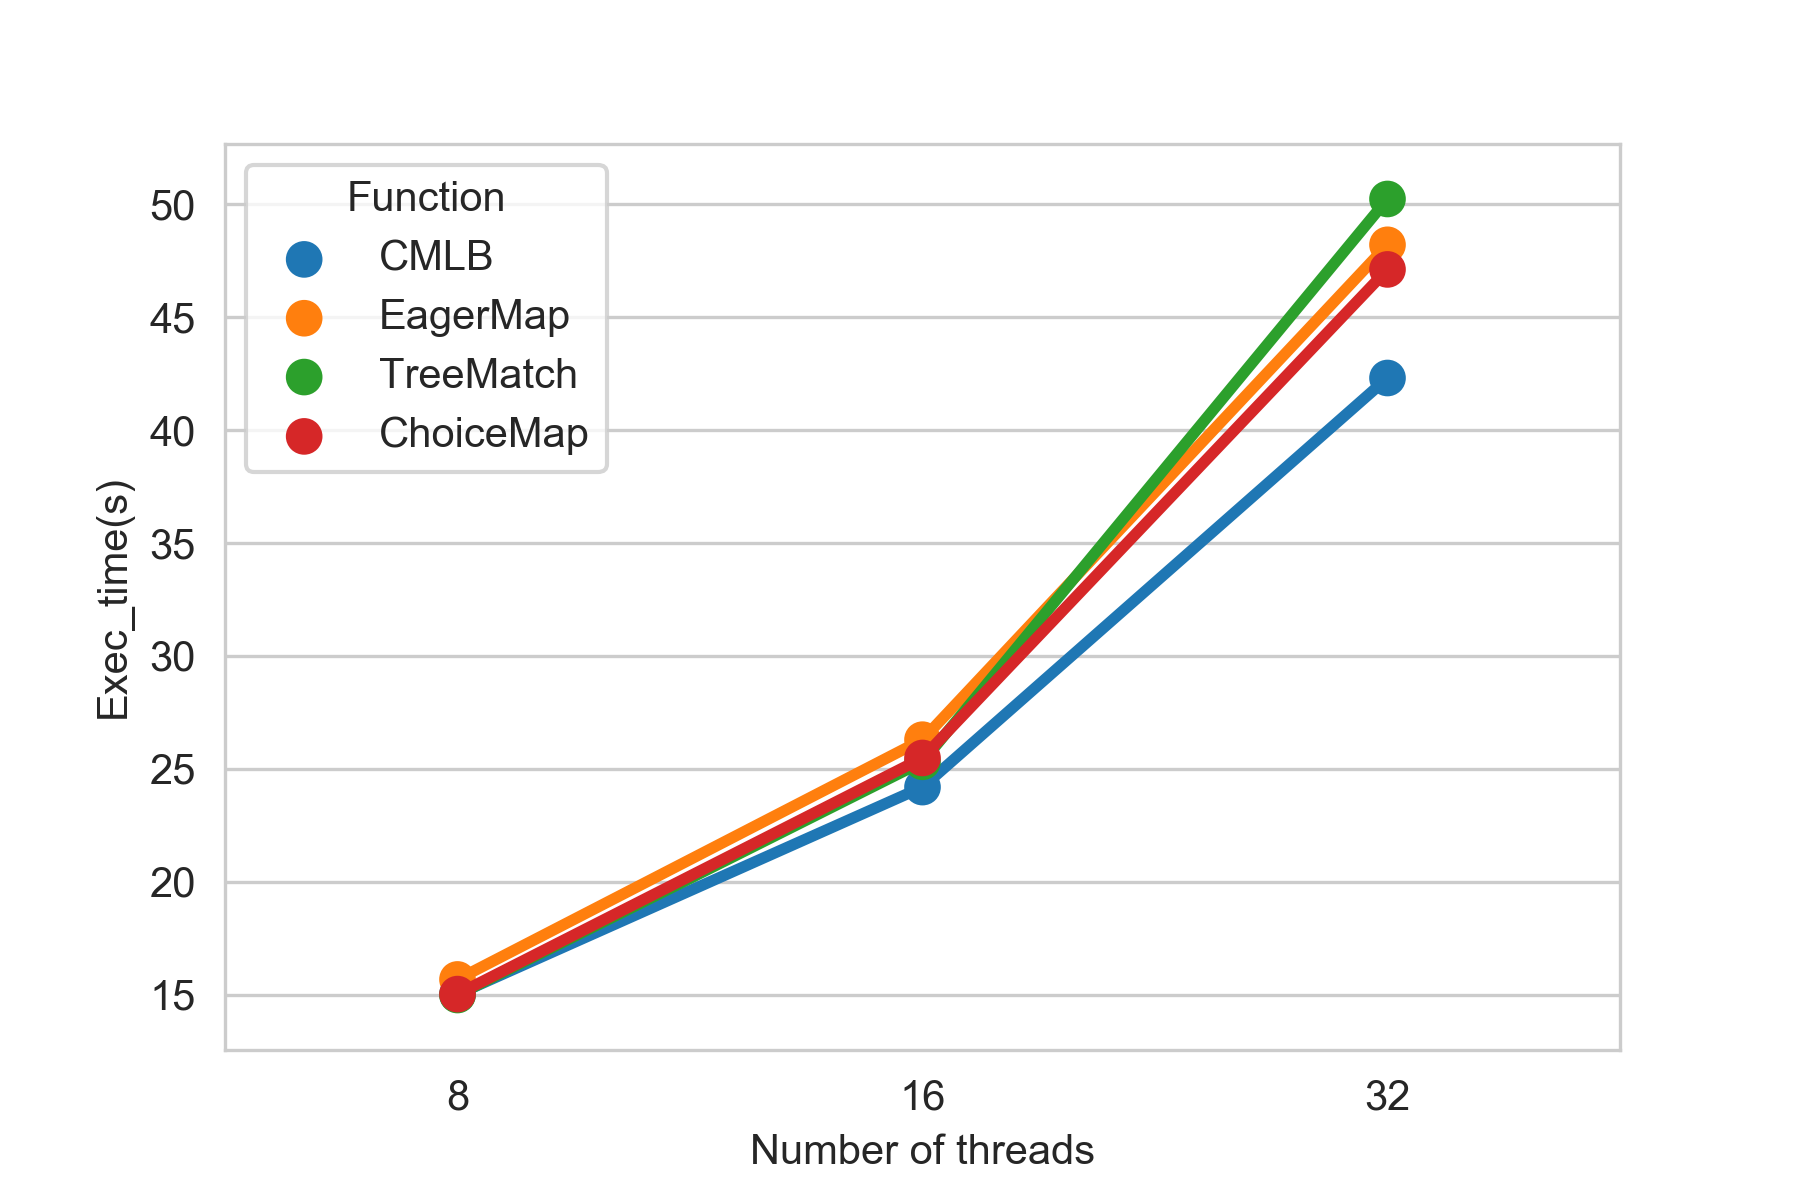
\includegraphics[scale=.40]{figs/Fig5a.png}
			%\caption{fig1}
		\end{minipage}%
	}%
	\subfigure[Average latency]{
		\begin{minipage}[t]{0.45\linewidth}
			\centering
			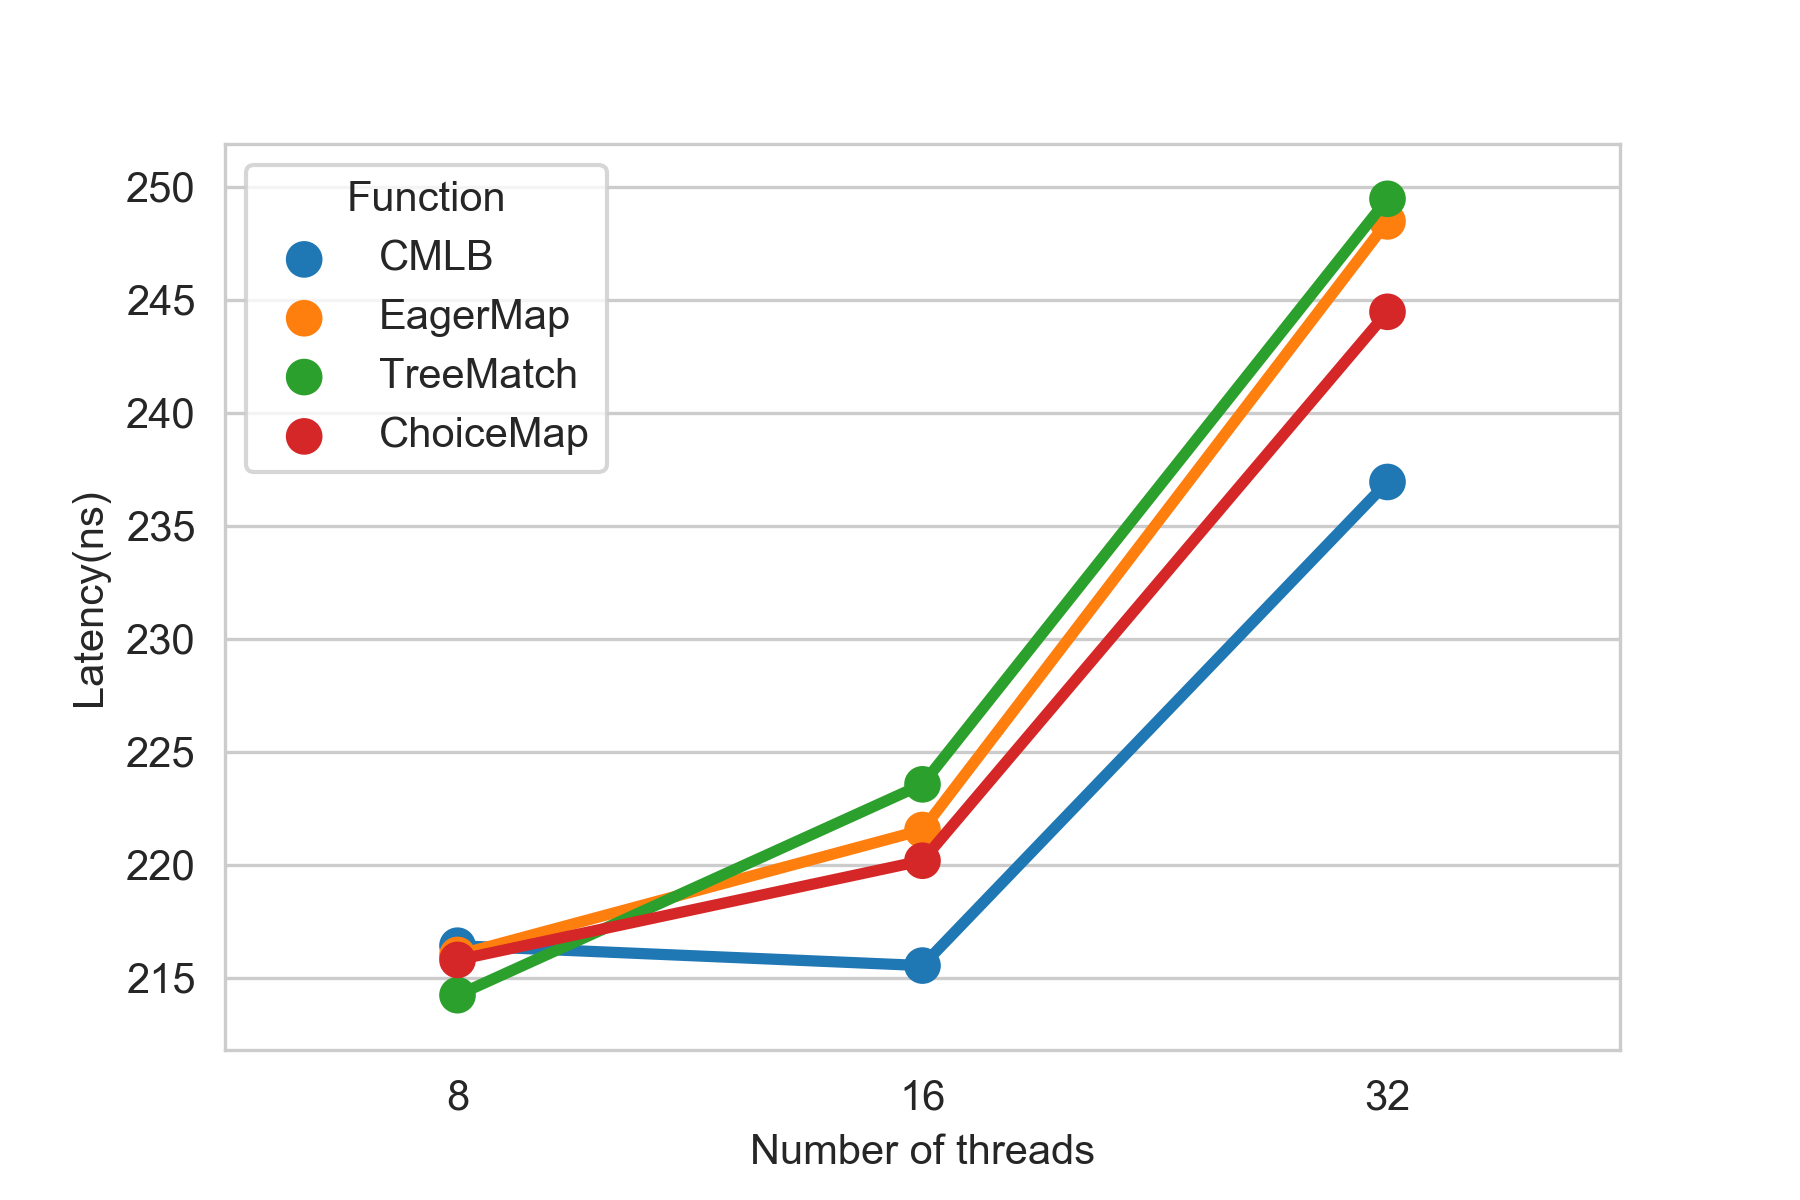
\includegraphics[scale=.40]{figs/Fig5b.png}
			%\caption{fig2}
		\end{minipage}%
	}%
	\, %这个回车键很重要 \quad也可以
	\subfigure[Imbalance of memory bandwidth]{
		\begin{minipage}[t]{0.45\linewidth}
			\centering
			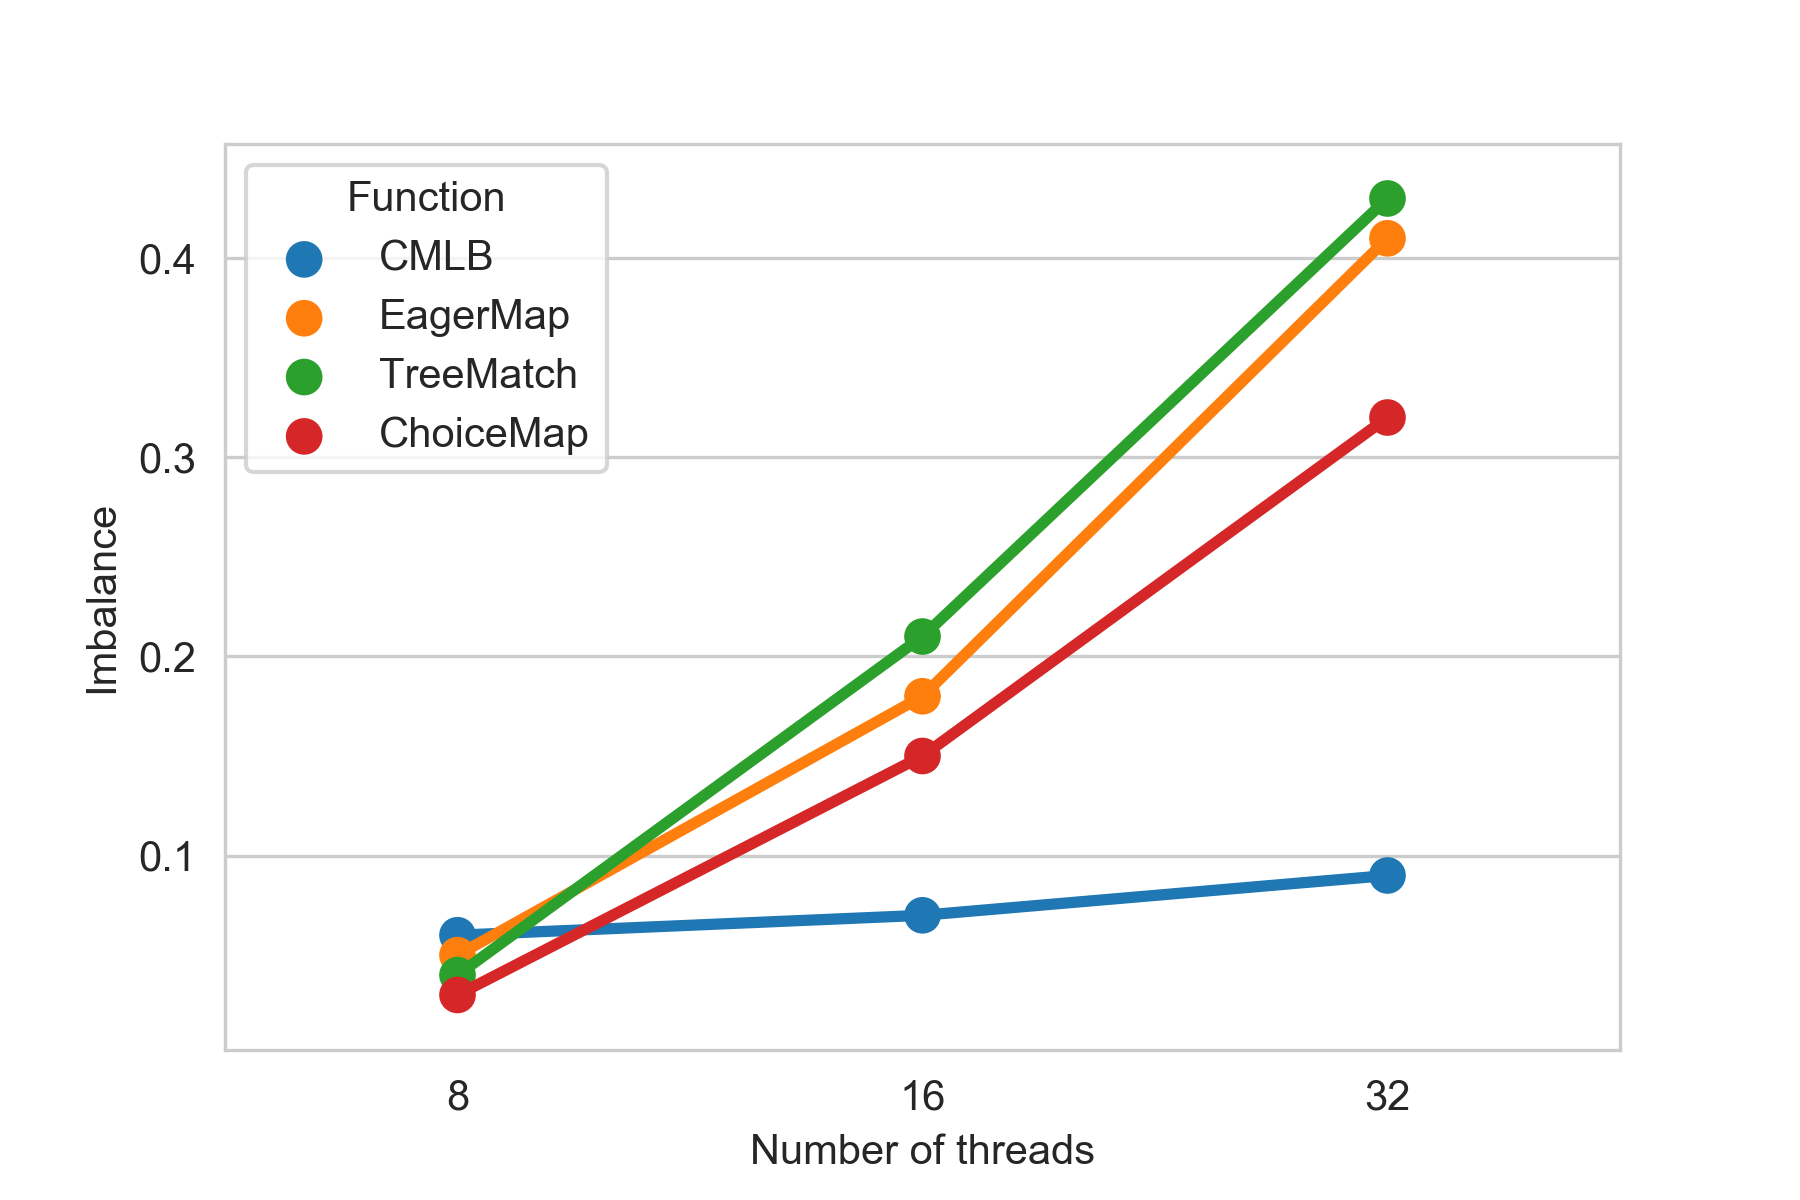
\includegraphics[scale=.40]{figs/Fig5c.png}
			%\caption{fig2}
		\end{minipage}
	}%
	\centering
	\caption{Experimental test on rotor35-omp} \label{FIG:5}
\end{figure}

The optimization performance of CMLB is more obvious when the number of threads is larger. As shown in Figure 4a, rotor35-omp with 32 threads have an obvious decrement about 6.25\% on execution time when comparing CMLB with the other mapping methods. For 8 and 16 threads versions of rotor35-omp, CMLB has the similar execution time with others. This is because the data size of rotor35-omp increases as the number of threads increases, and the number of memory accesses of the program also increases, resulting in an increasing in the remote communication and the imbalance of memory bandwidth between nodes. We also tested the imbalance of bandwidth between all nodes, which is measured by the variance of all the nodes memory bandwidth. As shown in Figure 4c, CMLB has the lowest value of the imbalance in the 16 and 32 threads rotor35, which indicates CMLB could balance the memory access load between all nodes better than the other methods, so that CMLB has the lowest average latency of rotor35 as shown in Figure 4b.
 
The above experiment shows that CMLB could balance the memory bandwidth between all the nodes and relieve the memory congestion problem which makes the average latency is significantly reduced, and finally make the execution time of rotor35-omp reduce. CMLB get the better performance on rotor35-omp than the other methods. 

\subsection{Test on NPB benchmark }
In this section, we use NPB benchmark to test the performance of CMLB. We selected SP, BT, LU and CG applications from NPB and test the performance from 4 metrics including execution time, QPI, the imbalance of memory bandwidth between nodes and the average latency, and for execution time, QPI, we compare that with the value before mapping. We tested the 4 applications with the Class B size and 32 threads. As shown in Figure 5, 
\begin{figure}[htbp] 
	\centering	
	\subfigure[Execution time improvement]{
		\begin{minipage}[t]{0.45\linewidth}
			\centering
			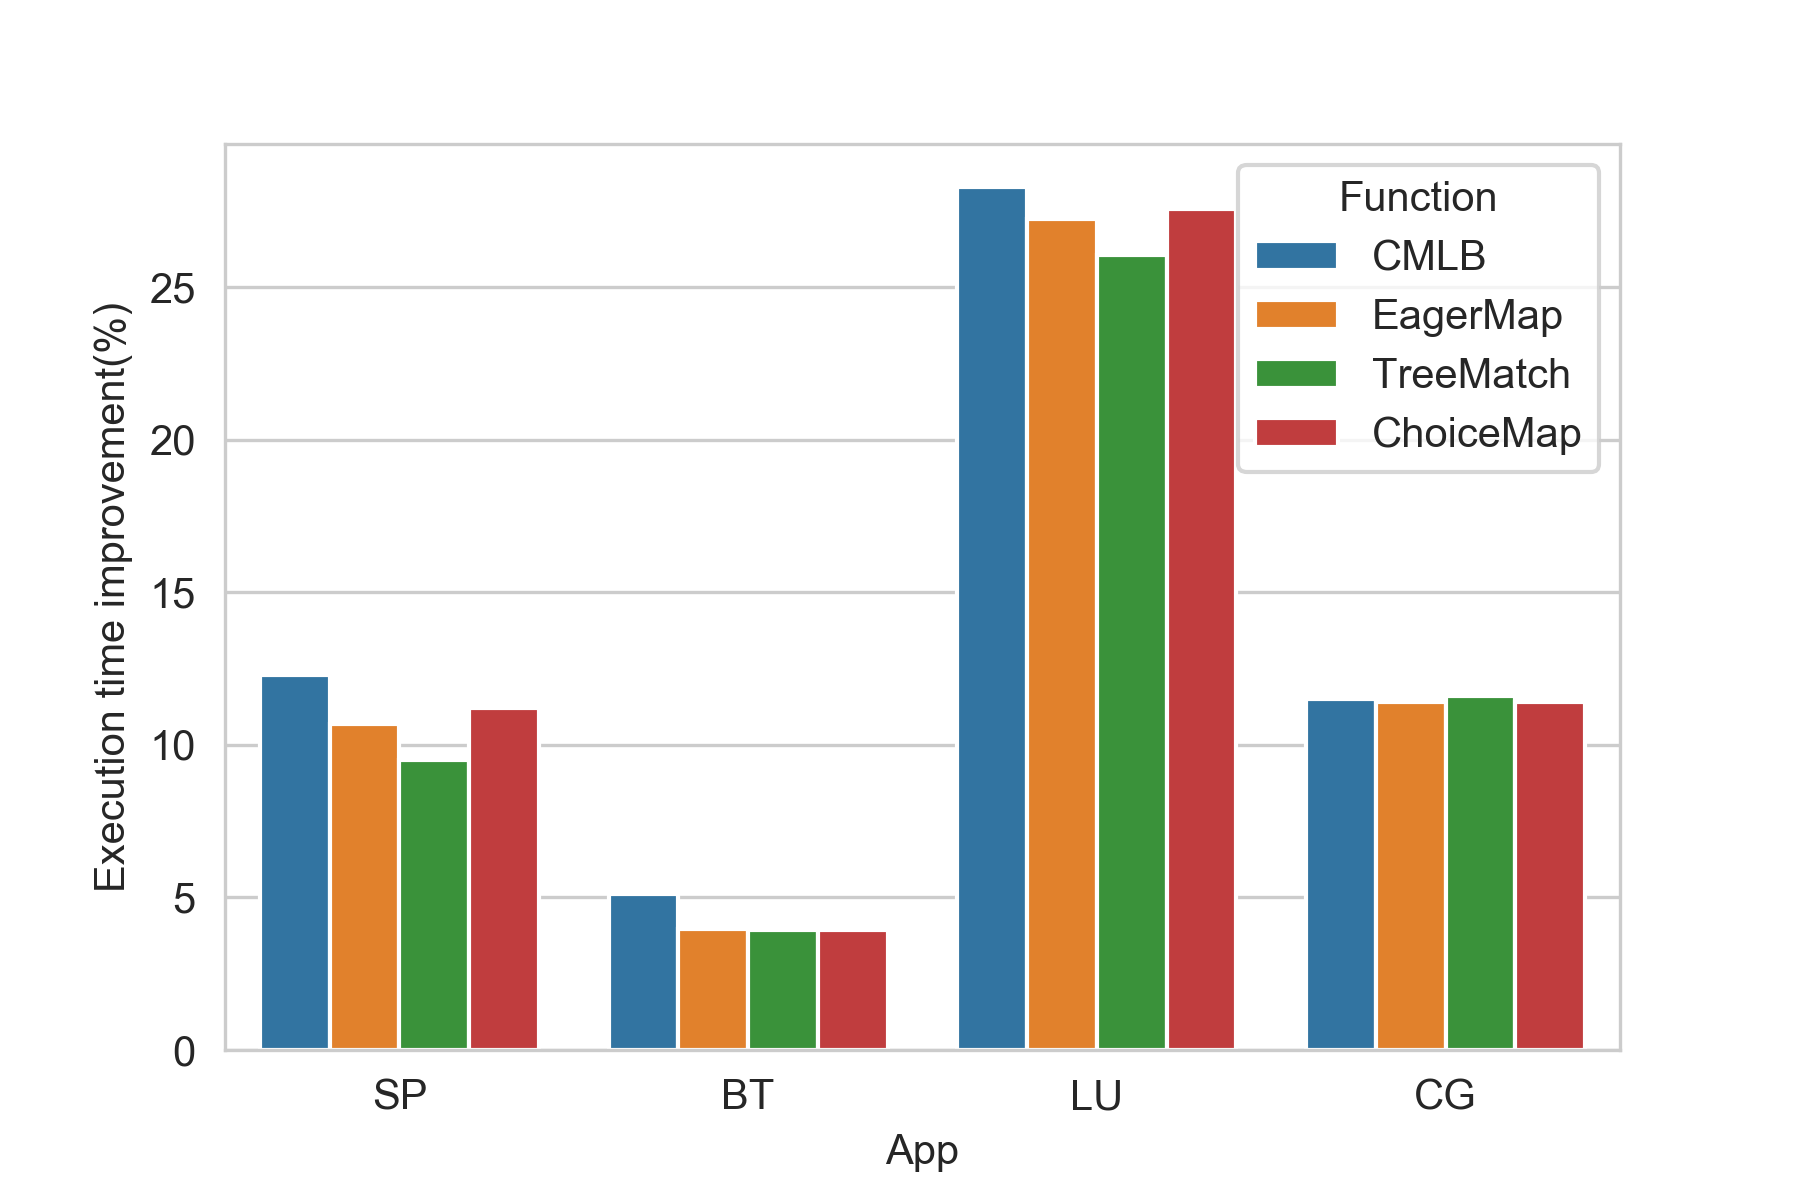
\includegraphics[scale=.40]{figs/Fig6a.png}
			%\caption{fig1}
		\end{minipage}%
	}%
	\subfigure[QPI improve]{
		\begin{minipage}[t]{0.45\linewidth}
			\centering
			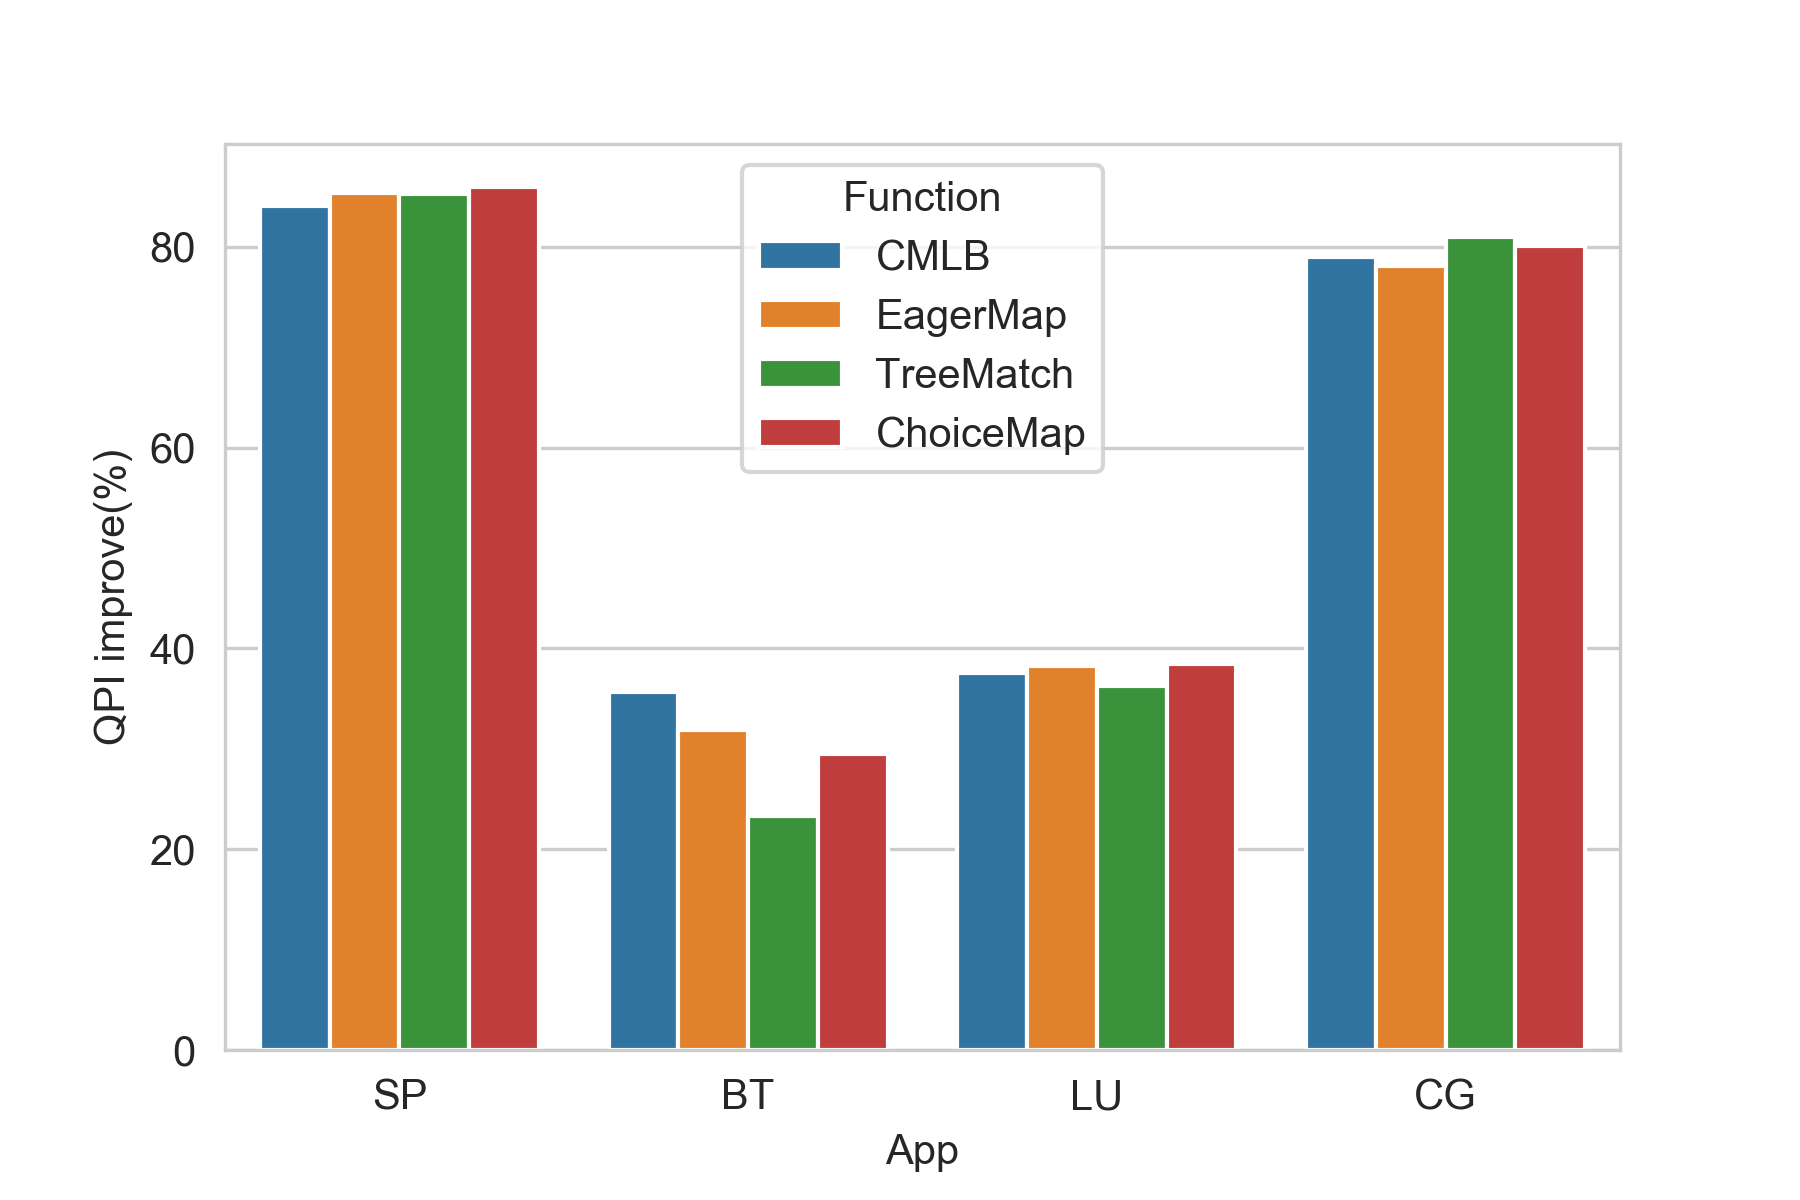
\includegraphics[scale=.40]{figs/Fig6b.png}
			%\caption{fig2}
		\end{minipage}%
	}%
	\, %这个回车键很重要 \quad也可以
	\subfigure[Imbalance of memory bandwidth]{
		\begin{minipage}[t]{0.45\linewidth}
			\centering
			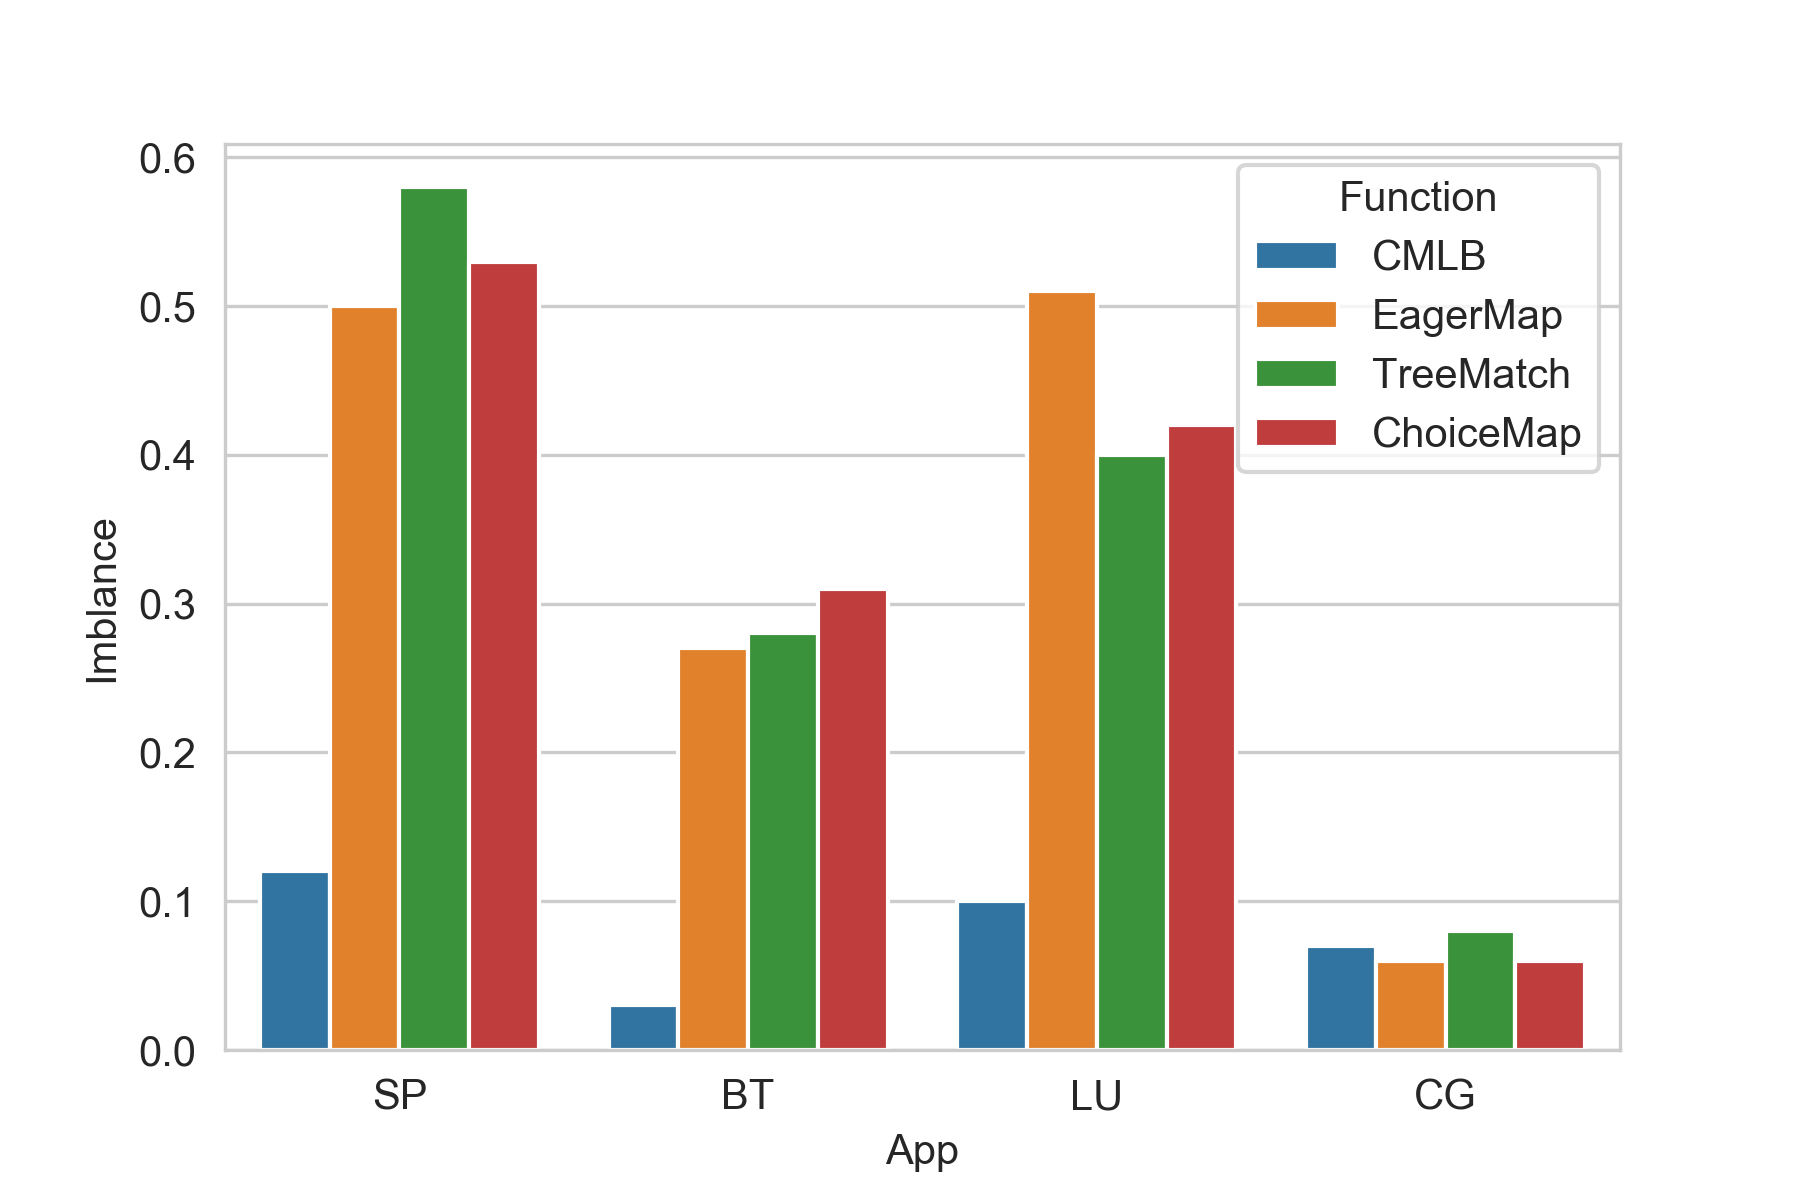
\includegraphics[scale=.40]{figs/Fig6c.png}
			%\caption{fig2}
		\end{minipage}
	}%
	\subfigure[Average latency]{
		\begin{minipage}[t]{0.45\linewidth}
			\centering
			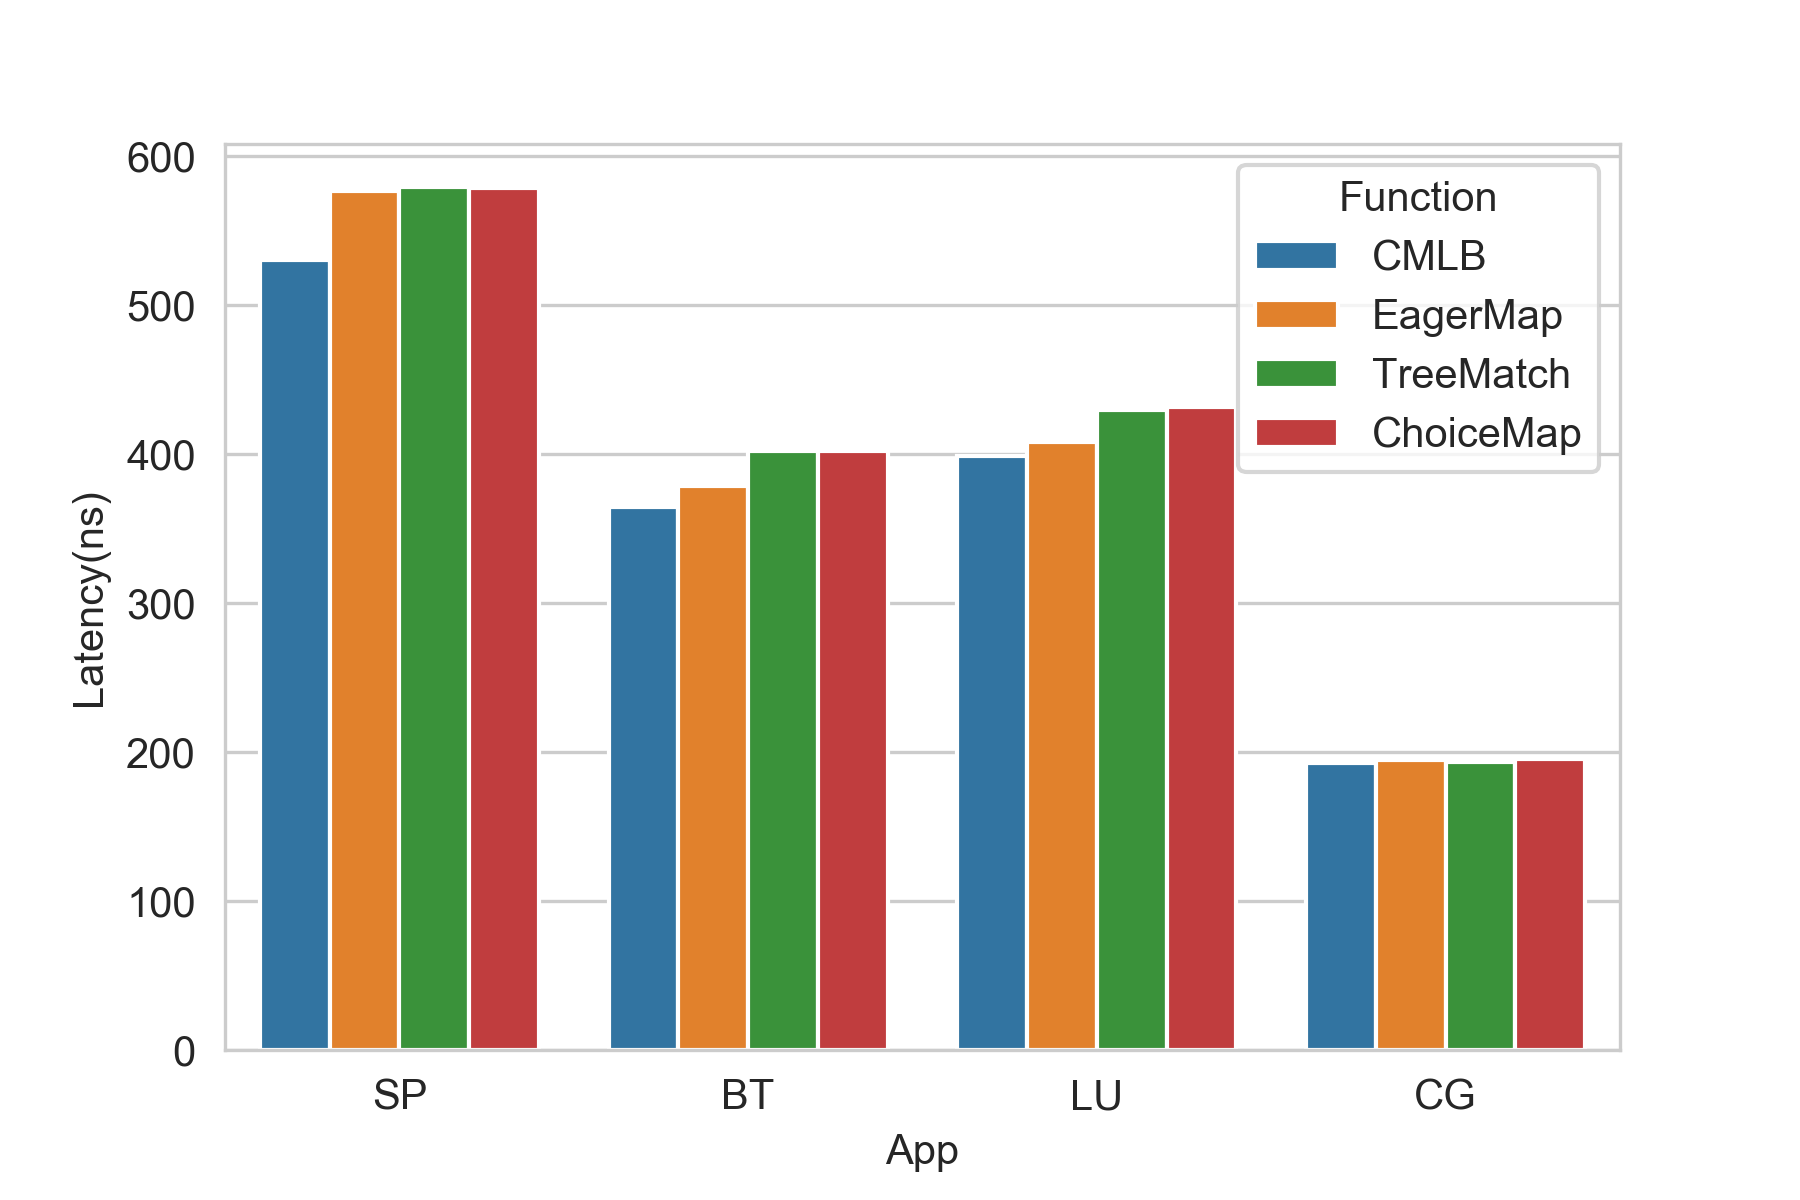
\includegraphics[scale=.40]{figs/Fig6d.png}
			%\caption{fig2}
		\end{minipage}%
	}%
	\centering
	\caption{Experimental test on NPB-OMP benchmark} \label{FIG:6}
\end{figure}
CMLB  has obvious optimization performance in SP, BT, LU, and CG applications compared to before mapping. The highest execution time improvement reaches about 28.29\%, and the highest QPI reduces about 84.03\%. Although CMLB is similar to EagerMap, TreeMatch and ChoiceMap in terms of QPI performance gains in SP, BT and LU applications, the imbalance of memory bandwidth is greatly reduced compared to other methods, BT has reduced significantly in that, compared with EagerMap, TreeMatch and ChoiceMap by about 88\%, 89\% and 92\%. And CMLB also reduce the average memory latency, the average memory latency of SP has reduced significantly, which is 8.1\%, 8.4\% and 8.3\% respectively compared with EagerMap, TreeMatch and ChoiceMap. The performance difference of the above metrics finally make the execution time improvement of the three applications SP, BT, and LU increase by 2.03\%, 2.20\% and 1.93\% on average compared to EagerMap, TreeMatch and ChoiceMap respectively.

As for CG, CMLB has not achieved any improvement in these metrics compared to other mapping methods. That is because the amount of memory access by each thread of CG is also roughly the same, and the memory bandwidth is always in a relatively balanced state, which make the average latency is also the same as other mapping methods.

Therefore, CMLB has a better optimization performance on the SP, BT, LU applications compared to EagerMap, TreeMatch and ChoiceMap. CMLB could greatly reduce the imbalance of memory bandwidth between all nodes and also reduce the amount of remote communication. Therefore, CMLB gain the best performance on execution time improvement which is also prove the theoretical evaluation in section 3.3.

\subsection{Test on Parsec benchmark }

We also used Parsec benchmark to test CMLB. And we selected Facesim, Streancluster and Fluidanimate applications with 32 threads from Parsec. As shown in Figure 6.



\begin{figure}[htbp] 
	\centering	
	\subfigure[Execution time improvement]{
		\begin{minipage}[t]{0.45\linewidth}
			\centering
			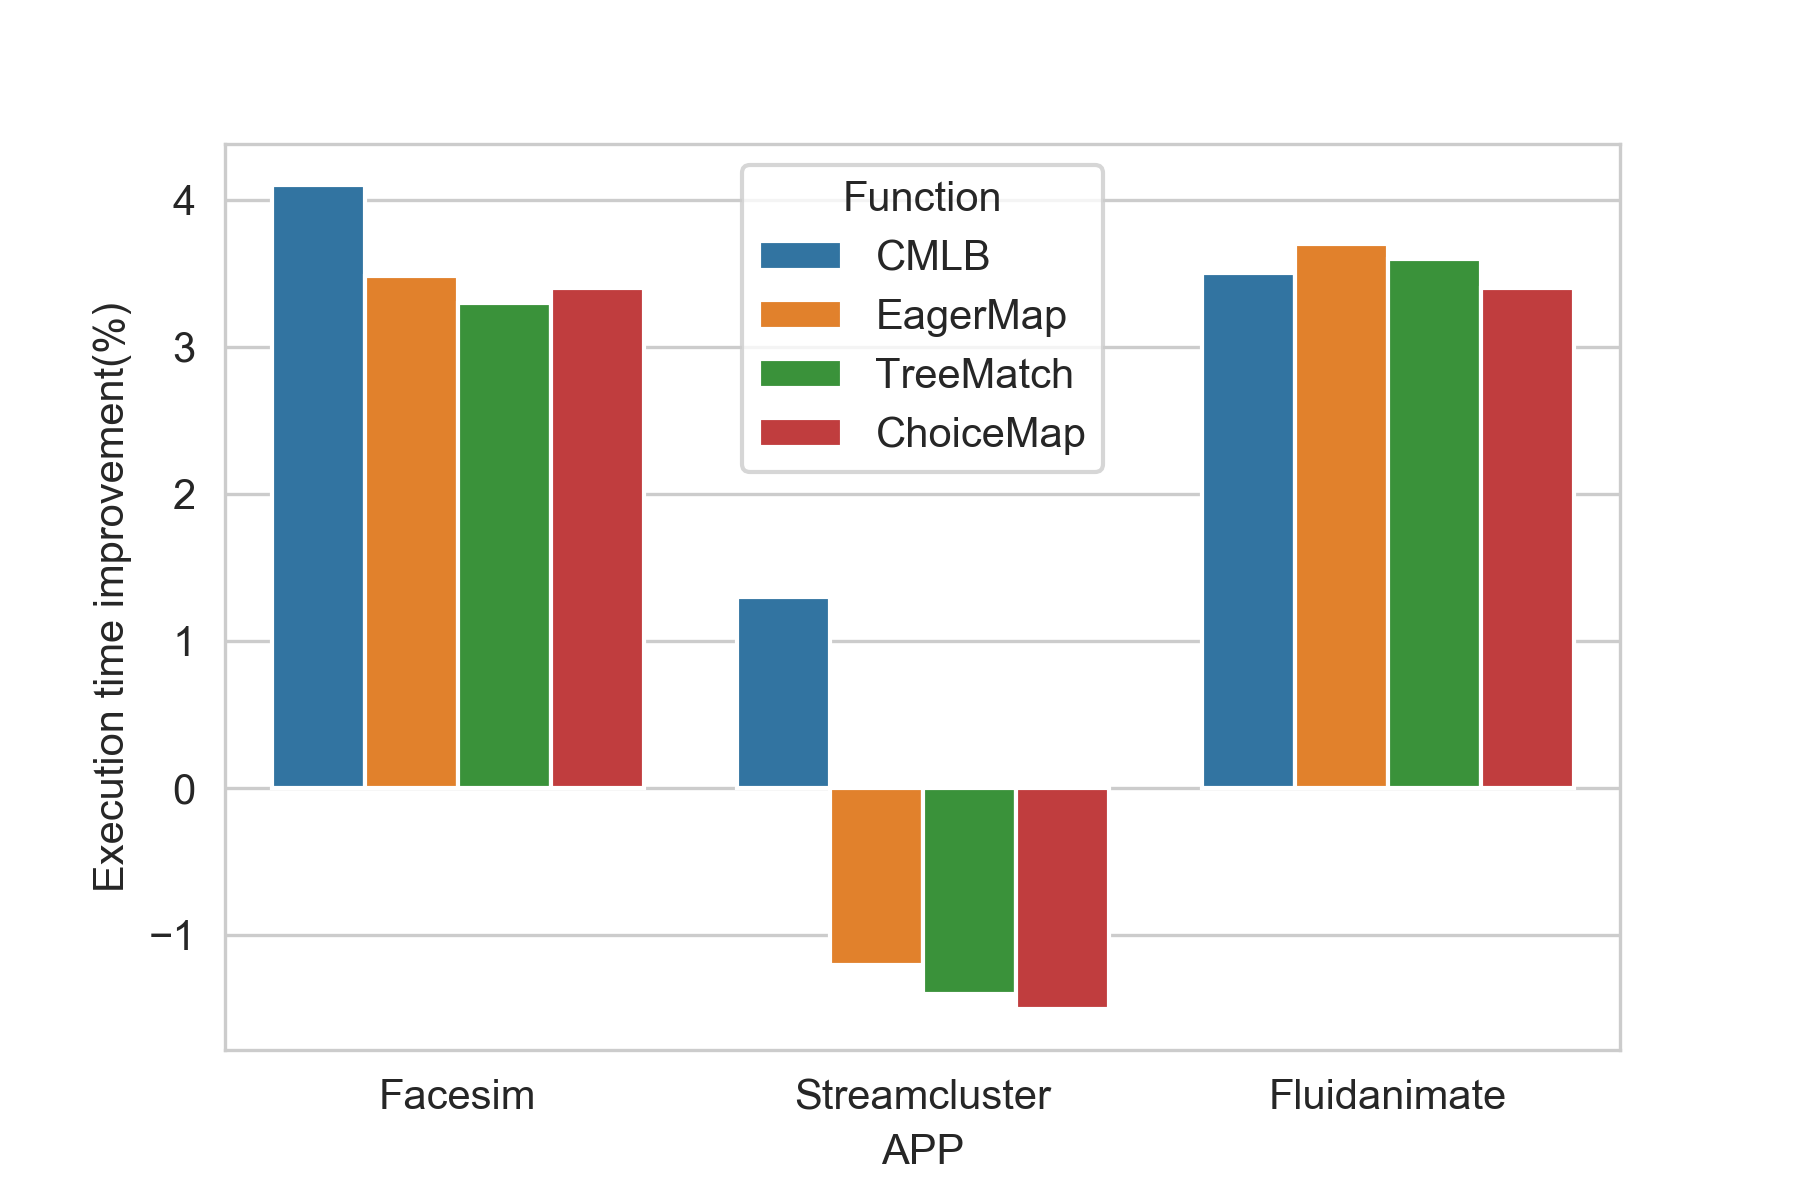
\includegraphics[scale=.40]{figs/Fig7a.png}
			%\caption{fig1}
		\end{minipage}%
	}%
	\subfigure[QPI improve]{
		\begin{minipage}[t]{0.45\linewidth}
			\centering
			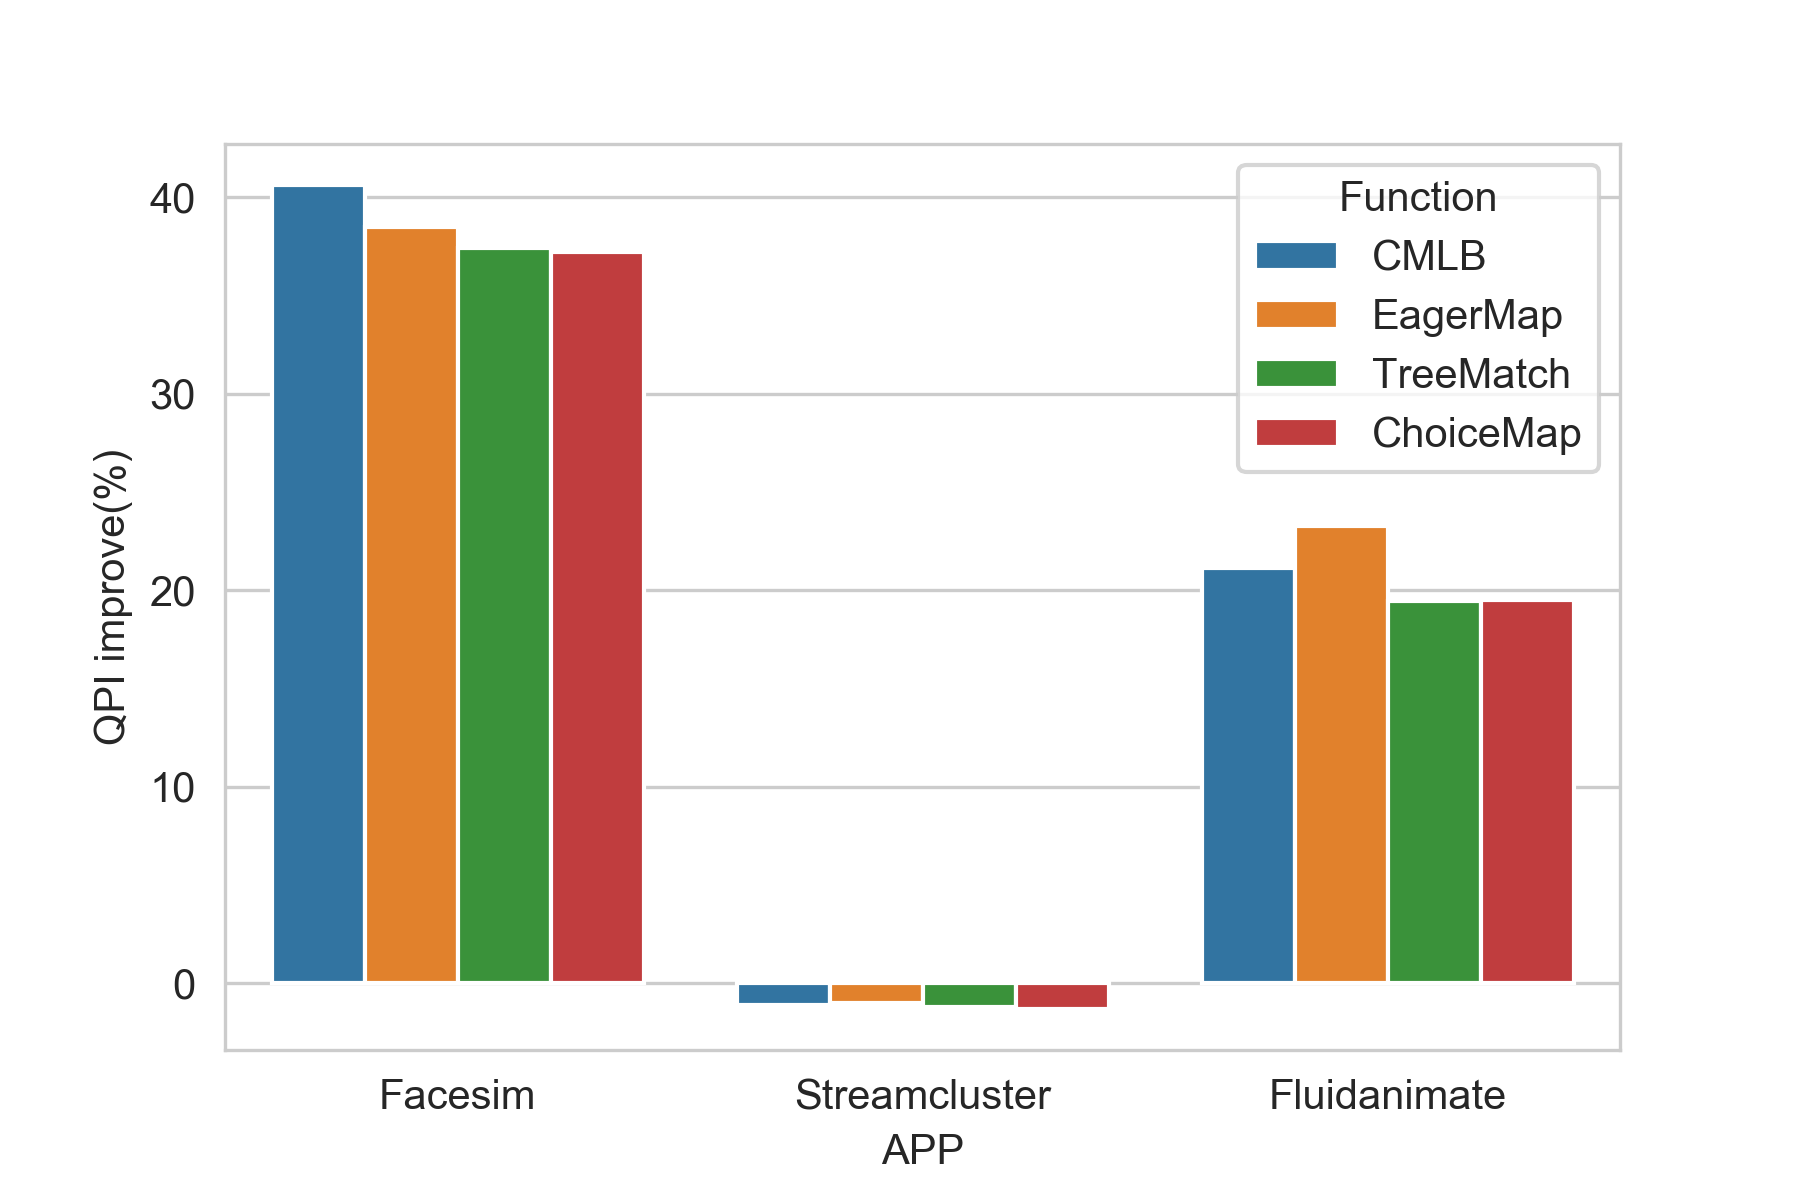
\includegraphics[scale=.40]{figs/Fig7b.png}
			%\caption{fig2}
		\end{minipage}%
	}%
	\, %这个回车键很重要 \quad也可以
	\subfigure[Imbalance of memory bandwidth]{
		\begin{minipage}[t]{0.45\linewidth}
			\centering
			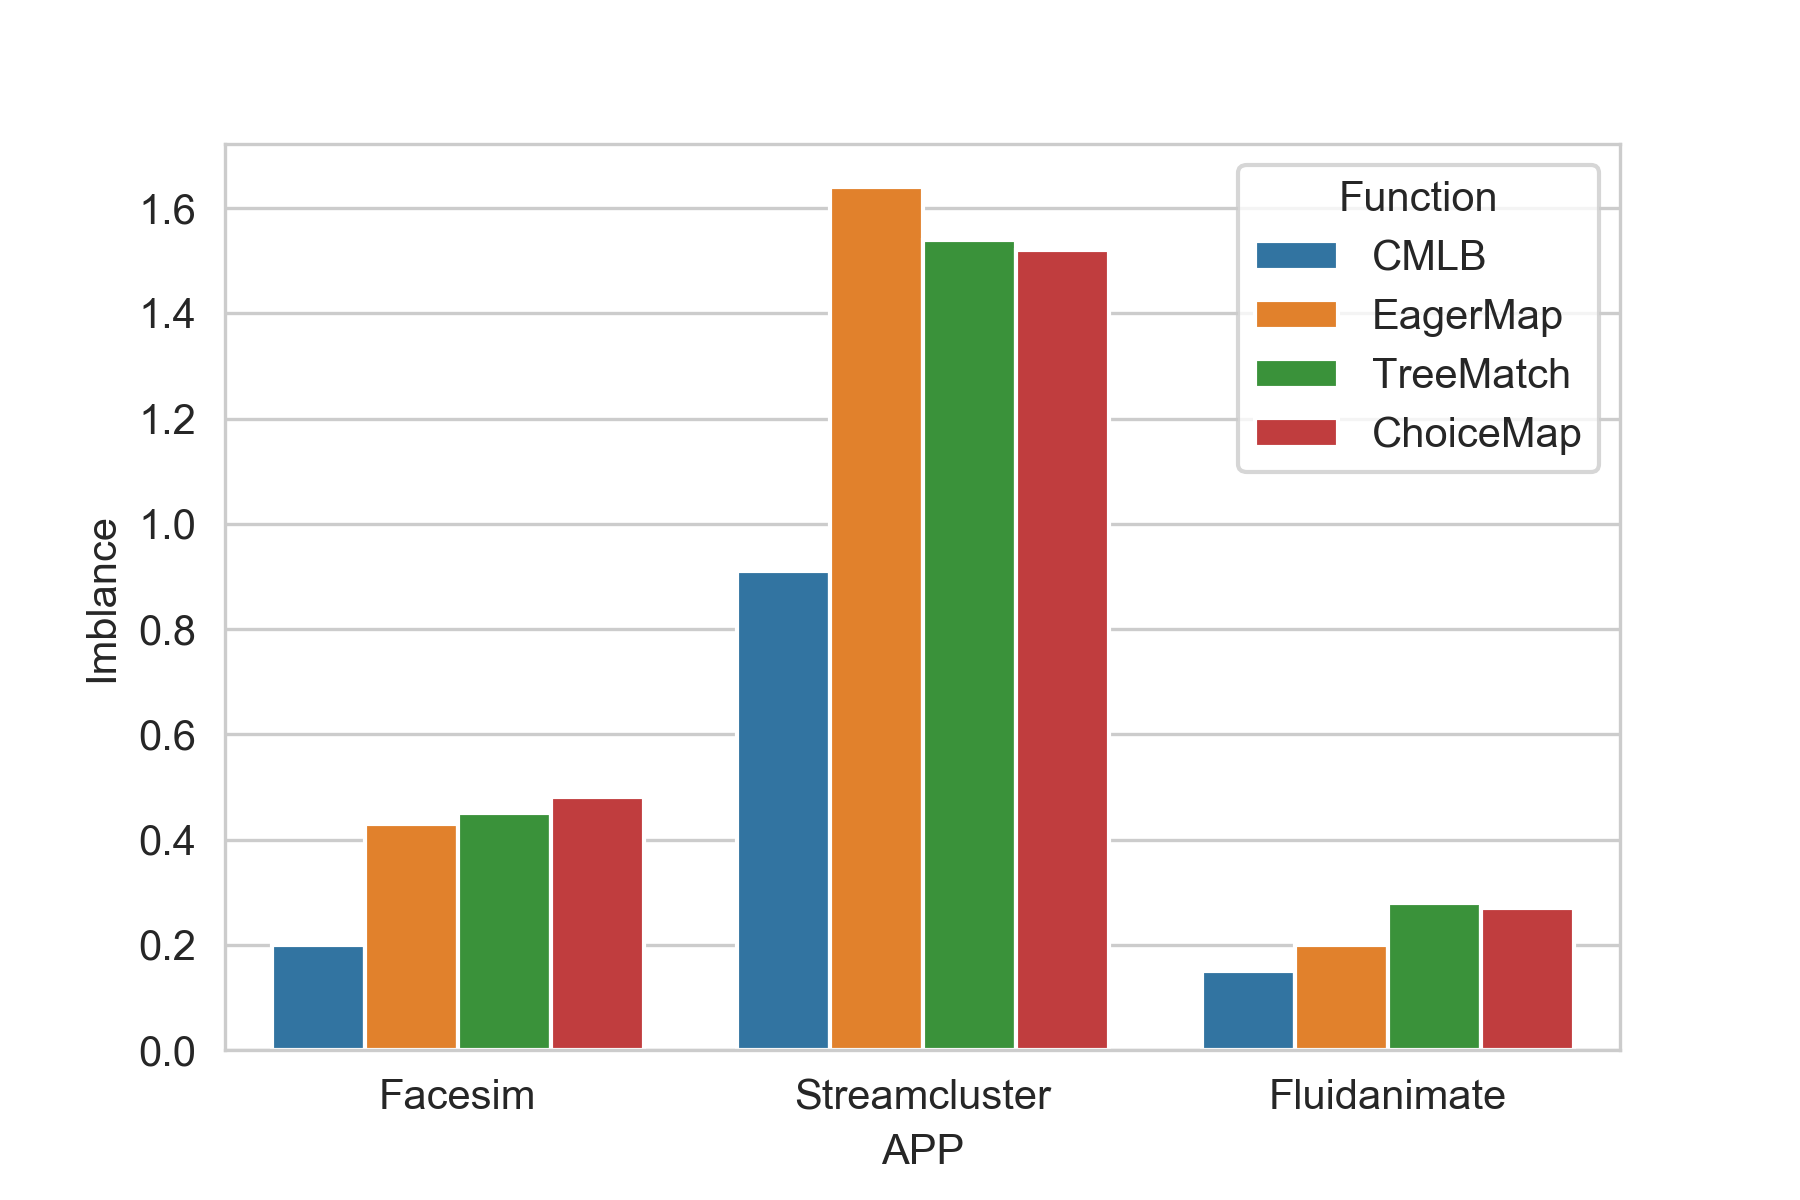
\includegraphics[scale=.40]{figs/Fig7c.png}
			%\caption{fig2}
		\end{minipage}
	}%
	\subfigure[Average latency]{
		\begin{minipage}[t]{0.45\linewidth}
			\centering
			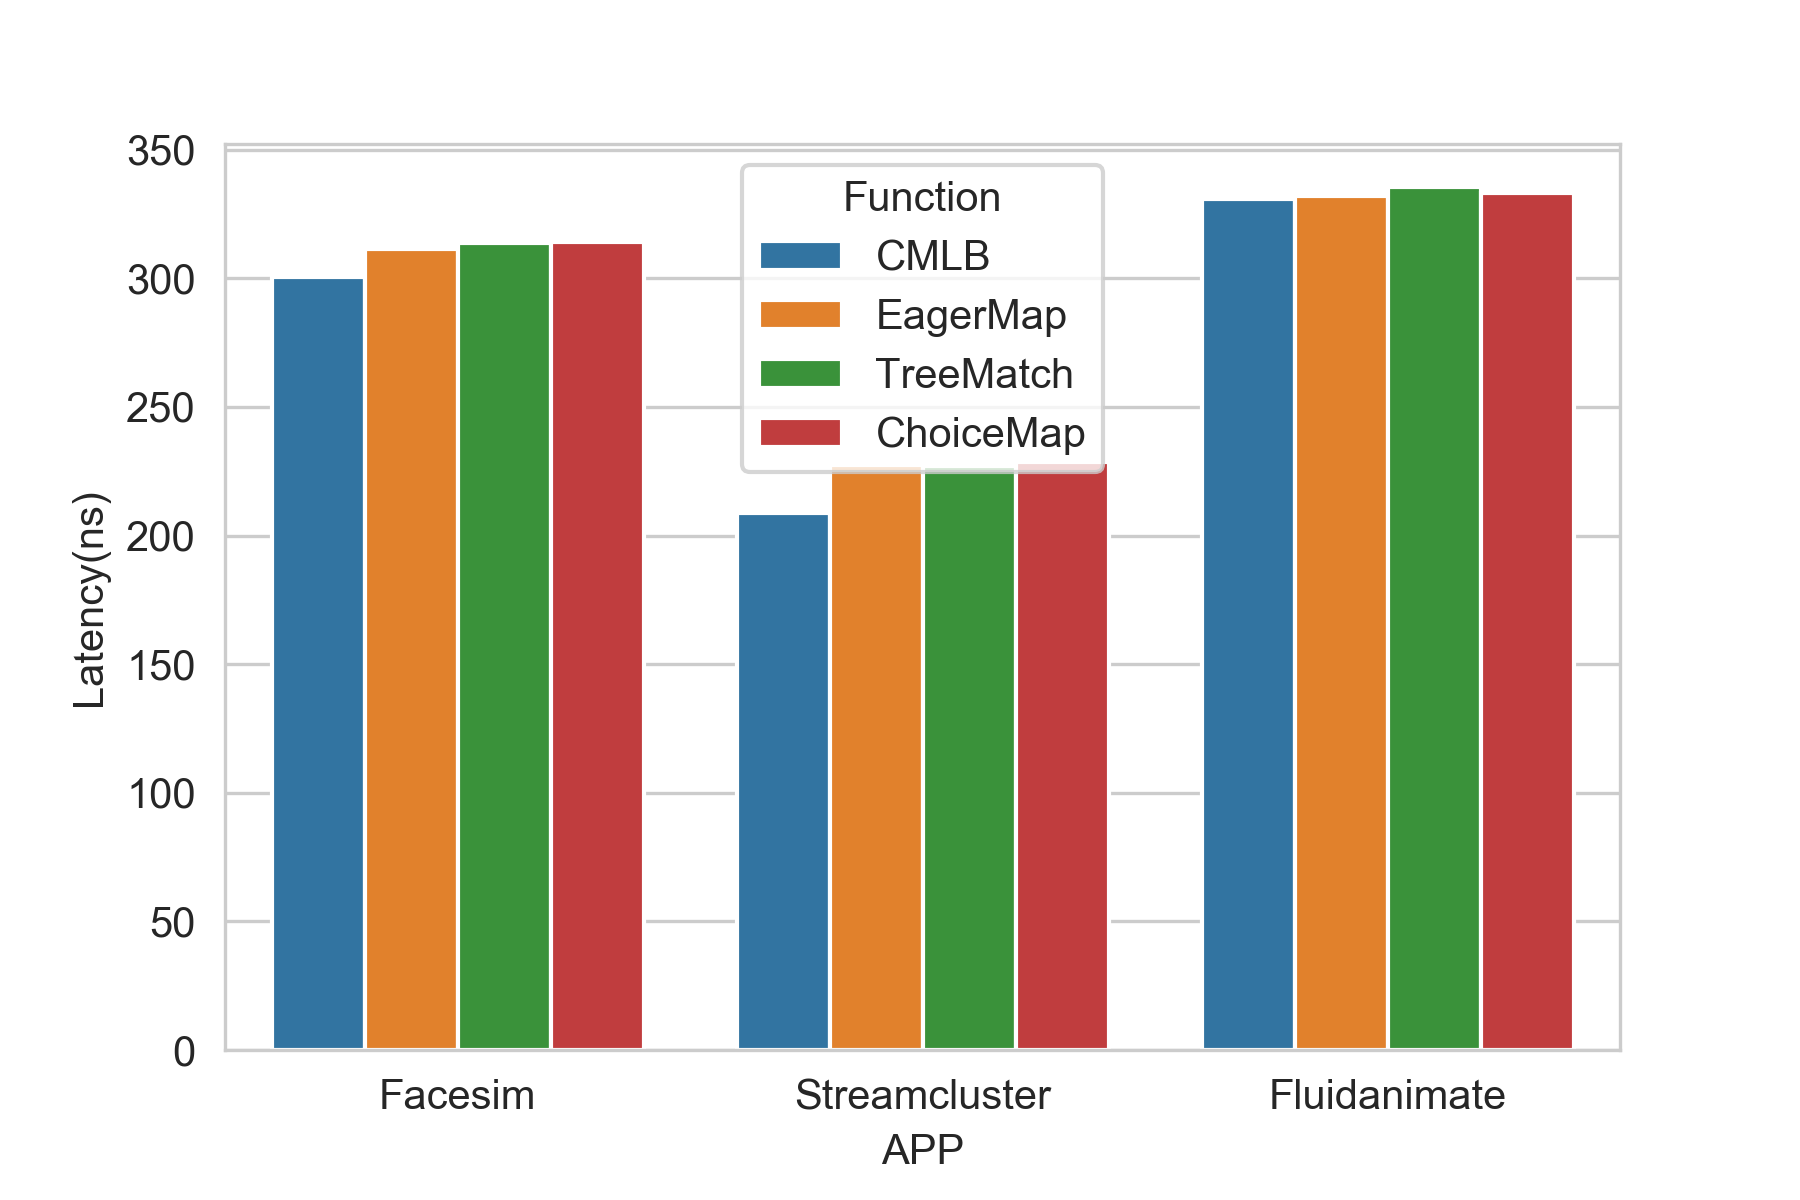
\includegraphics[scale=.40]{figs/Fig7d.png}
			%\caption{fig2}
		\end{minipage}%
	}%
	\centering
	\caption{Experimental test on Parsec benchmarks} \label{FIG:7}
\end{figure}

The test metrics are the same as NPB benchmark, CMLB has a certain optimization effect in Facesim, Streamcluster, and Fluidanimate compared to before mapping. The execution time improve is about 4.1\%, and the QPI is reduced about 40.1\% on average. When comparing with other methods, CMLB has the better performance on Facesim, Streamcluster applications than others. As for Streamcluster, CMLB reduce the imbalance of memory bandwidth about 2 times comparing with other methods, and also reduce about 8.3\% on average latency, so that make the execution time speed up about 1.3\% than before mapping.

For Fluidanimate application, it’s similar to CG. CMLB has the similar performance on QPI and the imbalance of memory bandwidth, so that the execution time of Fluidanimate has little difference among the 4 mapping methods.

Therefore, CMLB mapping method has a better optimization performance on the Facesim, Streancluster applications compared to EagerMap, TreeMatch and ChoiceMap, and has the similar performance on Fluidanimate.

\section{Conclusion} \label{sect5}
In parallel applications, mapping parallel tasks to cores according to the access behavior plays an important role to optimize the applications performance. By gathering and extracting the features of access behavior, and grouping threads according to that, the applications performance will get improved. 
In this paper, we proposed a new mapping method, CMLB. In contrast to previous work, it considers the access load of each thread, based on an analysis of the time series of access amount in an application. We performed experiments with rotor35-omp and several public applications with different access behavior. Results show that CMLB could improve the locality of communication between threads and balance the memory bandwidth between nodes, greatly relieve the memory congestion problem and get the better performance than the state-of-the-art. 
For the future, we will extend CMLB to map tasks on a heterogeneous platform including both CPUs and GPUs.
\section{Declaration of competing interest}
The authors declare that they have no known competing financial interests or personal relationships that could have appeared to influence the work reported in this paper.

\section{Acknowledgments}
This research was funded by the National Key Research and Development Program of China, grant number: 2016YFB0200902.

%% Loading bibliography style file
\bibliographystyle{model1-num-names}
\bibliographystyle{cas-model2-names}
\bibliographystyle{plain}
\bibliographystyle{unsrt}

\makeatletter
\renewcommand{\@biblabel}[1]{[#1]}
\makeatother

\begin{thebibliography}{70}

\bibitem{1}D. Molka, D. Hackenberg, and R. Schöne, “Main Memory and Cache Performance of Intel Sandy Bridge and AMD Bulldozer,” in Proceedings of the Workshop on Memory Systems Performance and Correctness, ser. MSPC ’14. New York, NY, USA: ACM, 2014, pp. 4:1–4:10.
\bibitem{2}F. Gaud, B. Lepers, J. Funston, M. Dashti, A. Fedorova, V. Quéma, R. Lachaize, and M. Roth, “Challenges of Memory Management on Modern NUMA Systems,” Queue, vol. 13, no. 8, p. 70, 2015.
\bibitem{3}M.Diener,E.H.Cruz,M.A.Alves,P.O.Navaux,andI.Koren,“Affinity- based thread and data mapping in shared memory systems,” ACM Com- puting Surveys (CSUR), vol. 49, no. 4, p. 64, 2017.
\bibitem{4}D.Ziakas,A.Baum,R.A.Maddox,andR.J.Safranek,“IntelQuickPath Interconnect Architectural Features Supporting Scalable System Architec- tures,” in 2010 18th IEEE Symposium on High Performance Interconnects, Aug 2010, pp. 1–6.
\bibitem{5}E. H. M. Cruz, M. Diener, LL. Pilla, P. O. A. Navaux, An efficient algorithm for communication-based task mapping. Paper presented at: 2015 23rd Euromicro International Conference on Parallel, Distributed and Network-Based Processing (PDP); 2015; Turku, Finland.
\bibitem{6}E. H. M. Cruz, M. Diener, M. A. Z. Alves, and P. O. A. Navaux, “Dynamic thread mapping of shared memory appli- cations by exploiting cache coherence protocols,” Journal of Parallel and Distributed Computing, vol. 74, no. 3, 2014.
\bibitem{7}M. Dashti, A. Fedorova, J. Funston, F. Gaud, R. Lachaize, B. Lepers, V. Quema, and M. Roth, “Traffic management: a holistic approach to memory placement on NUMA systems,” in ACM SIGPLAN Notices, vol. 48, no. 4. ACM, 2013, pp. 381–394.
\bibitem{8}S. Ito, K. Goto, and K. Ono, “Automatically optimized core mapping to subdomains of domain decomposition method on multicore parallel environments,” Computers & Fluids, vol. 80, pp. 88–93, Jul. 2013.
\bibitem{9}K. D. Devine, E. G. Boman, R. T. Heaphy, R. H. Bissel- ing, and U. V. Catalyurek, “Parallel hypergraph partitioning for scientific computing,” in IEEE International Parallel & Distributed Processing Symposium (IPDPS), 2006.
\bibitem{10}F. Pellegrini, “Static Mapping by Dual Recursive Bipartition- ing of Process and Architecture Graphs,” in Scalable High- Performance Computing Conference (SHPCC), 1994.
\bibitem{11}E. Jeannot, G. Mercier, and F. Tessier, “Process Placement in Multicore Clusters: Algorithmic Issues and Practical Tech- niques,” IEEE Transactions on Parallel and Distributed Sys- tems, vol. 25, no. 4, pp. 993–1002, Apr. 2014
\bibitem{12}E. H. M. Cruz, M. Diener, LL. Pilla, P. O. A. Navaux, EagerMap: A Task Mapping Algorithm to Impromove Communication and Load Balancing in Clusters of Multicore Systems. ACM Transactions on Parallel Computing, 2019, 5(4), pp. 1-24.
\bibitem{13}P. N. Soomro, M. A. Sasongko, D. Unat. BindMe: A thread binding library with advanced mapping algorithms. Concurrency Computat Pract Exper (cpe), vol.30, no. 21, p.e4692, 2018.

\bibitem{14}M. Diener, E. H. M. Cruz, LL. Pilla, P. O. A. Navaux, Communication in shared memory: Concepts, definitions, and efficient detection. Paper presented at: 2016 24th Euromicro International Conference on Parallel, Distributed, and Network-Based Processing (PDP); 2016; Heraklion, Greece.
\bibitem{15}V. J. Reddi, A. Settle, D. A. Connors, R. S. Cohn. PIN: a binary instrumentation tool for computer architecture research and education. In: Proceedings of the 2004 Workshop on Computer Architecture Education: Held in Conjunction with the 31st International Symposium on Computer Architecture; 2004; Munich, Germany.
\bibitem{16}M. A. Sasongko, M. Chabbi, P. Akhtar, and D. Unat. 2019. ComDetective: A Lightweight Communication Detection Tool for Threads . In Proceedings of ACM Supercomputing (SC’19). ACM, New York, NY, USA, 12 pages.
\bibitem{17}Long DL, Clarke LA. Task interaction graphs for concurrency analysis. In: Proceedings of the 11th International Conference on Software engineering; 1989; Pittsburgh, PA.
\bibitem{18}Intel. 2010. Intel Microarchitecture Codename Nehalem Performance Monitoring Unit Programming Guide. https://software.intel.com/sites/default/files/m/5/2/c/ f/1/30320- Nehalem- PMU- Programming- Guide- Core.pdf .
\bibitem{19} L. Zhihan, Z. Youjian, L. Rong, et al. Robust and Rapid Clustering of KPIs for Large-Scale Anomaly Detection//IEEE/ACM 26th International Symposium on Quality of Service(IWQoS), Banff, AB, Canada, 2018: 1-10.
\bibitem{20}F  Broquedis, J Clet-Ortega, S Moreaud, et al. hwloc: A generic framework for managing hardware affinities in HPC applications. Paper presented at: 2010 18th Euromicro International Conference on Parallel, Distributed and Network-Based Processing (PDP); 2010; Pisa, Italy.
\end{thebibliography}



%\section{References}


% Loading bibliography database


%\appendix
%\section{Appendix}




\end{document}

